% Created 2017-12-16 Sat 10:23
\documentclass[11pt]{article}
\usepackage[utf8]{inputenc}
\usepackage[T1]{fontenc}
\usepackage{fixltx2e}
\usepackage{graphicx}
\usepackage{grffile}
\usepackage{longtable}
\usepackage{wrapfig}
\usepackage{rotating}
\usepackage[normalem]{ulem}
\usepackage{amsmath}
\usepackage{textcomp}
\usepackage{amssymb}
\usepackage{capt-of}
\usepackage{hyperref}
\usepackage{amsmath}
\usepackage{amssymb}
\author{Jack Truskowski}
\date{\today}
\title{CS640: Introduction to Computer Networks Notes}
\hypersetup{
 pdfauthor={Jack Truskowski},
 pdftitle={CS640: Introduction to Computer Networks Notes},
 pdfkeywords={},
 pdfsubject={},
 pdfcreator={Emacs 24.5.1 (Org mode 8.3.5)}, 
 pdflang={English}}
\begin{document}

\maketitle
\tableofcontents


\section{9/7/17  History of Communication}
\label{sec:orgheadline3}
\begin{itemize}
\item Python environment called Switchyard
\end{itemize}
\subsection{Communication}
\label{sec:orgheadline1}
\begin{itemize}
\item Spoken language \textasciitilde{} 100k years ago
\item Written language \textasciitilde{} 8000 BC
\item Carrier Systems \textasciitilde{} 2400 BC

\item Telegraph/Morse - 1837
\begin{itemize}
\item (Virtually) Instantaneous Communication
\end{itemize}

\item Telephone - 1875
\item Film/TV/Radio - 1894/1927/1896
\end{itemize}

\subsection{Internet History (Machine-to-Machine Communication)}
\label{sec:orgheadline2}
Telephone Network -> Circuit switching
\begin{itemize}
\item C. Shannon ('40s)
\item circuit switching  have to have a set of wires that connect you and only you to remote entity
\item circuit switching is not a robust infrastructure (can't handle small
disruptions)
\end{itemize}

1905s: 3 groups working on 'packet switching'
\begin{itemize}
\item Beren, Kleinrock, Davies
\item Makes system more robust to outage
\item Greater efficiency
\end{itemize}

1967 - ARPHnet (by the Government)
\begin{itemize}
\item plan for the first packet switched network
\end{itemize}

1969 - First 4-node ARPAnet (UCLA, SRI, UCSB, Utah)
\begin{itemize}
\item V. Cerf, R. Kahn, L. Roberts
\item First application = Rlogin (remote login)
\end{itemize}

1972 - 15 nodes, RFC (request for comment) 001 = Network Control Protocol
\begin{itemize}
\item Facilitates consistency and inter-operability among a community of participants
\item ICANN -> John Postal
\item R. Tomlinson invents \textbf{email}
\end{itemize}

1973 - Ethernet
1974 - TCP/IP

1989 - 100k nodes
\begin{itemize}
\item V. Jacobson enhances TCP
\item Invention of DNS (Domain name system)
\end{itemize}

1991 - HTTP invented (Tim Berners-Lee)
1993 - MOSAIC (graphical browser) invented (M. Andreeson)

1999 - Napster
\begin{itemize}
\item Google \textasciitilde{}2000
\item Facebook 2004
\end{itemize}

2007 - iPhone

\section{9/12/17  Network Basics and 3 Perspectives on Networks}
\label{sec:orgheadline6}
Perspectives:
\begin{enumerate}
\item Abstract
\item Internet
\item Architectural
\end{enumerate}

\subsection{Basics (Abstract Perspective)}
\label{sec:orgheadline4}
\begin{itemize}
\item Nodes = Devices that facilitate communication (end-node, client)
eg) computers, phones, routers, switches, and more
\item Links = A physical medium that facilitates the transmission of
signals
\end{itemize}



\textbf{Point-to-Point Network:}

\begin{verbatim}
  [Comp] - [Comp] 
           ^ protocol (eg PPP)
\end{verbatim}

\begin{itemize}
\item Full Duplex Communication: allows 2-way communication at the same
time
\end{itemize}



\textbf{Multiple Access:}

\begin{verbatim}
[Comp] [Comp] [Comp]
   \|-/ 
              ^shared medium (bus)
\end{verbatim}

\begin{itemize}
\item Not \textbf{scalable}
\end{itemize}



\textbf{Switched:}

\begin{verbatim}
            [comp]
{             |
[router] - [router] - [comp]  
      \      /
      [router] - [comp]
} <-represents more infrastructure
\end{verbatim}

\begin{itemize}
\item Intermediate nodes enable scaling
\item More than 2 nodes can communicate at the same time

\item Circuit Switching:
\item Establish a dedicated path between end nodes via signaling after which communication = stream of bits
\item Packet Switching:
\item Data is divided into packets (discrete blocks) and sent in shared environment toward the destination using \textbf{store and forward} nodes
\item Robustness
\item Efficient resource utilization
\end{itemize}



\textbf{Network of Networks}

\begin{verbatim}
{}  {} - [comp]
  \  / <- Must enable communication between variety of networks
   {} - [comp]
\end{verbatim}

\begin{itemize}
\item This is \textbf{The Internet} (a network of networks)

\item \textbf{Address}: Unique identifier which enables nodes to be targeted. Internet uses 'destination-based forwarding' to send packets
\^{} destination address in packets
\item \textbf{Forwarding} Facilitated by nodes that are not directly connected to
destination nodes. 
\^{} process based on table lookups in store and forward devices. Results in transmitting packet on outgoing link
\item \textbf{Routing}: process for establishing forwarding tables in routers.
\item \textbf{Multiplexing}: sharing a resource among multiple entities
eg) TDM (time division multiplexing), FDM (frequency division
multiplexing)
\begin{itemize}
\item \textbf{Statistical Multiplexing}:
\end{itemize}
\end{itemize}

\begin{verbatim}
    Inputs -> 
           -> [queue+server] -> Output
           ->
\end{verbatim}

\begin{itemize}
\item There is some policy for aggregating packets as they come into
these devices
\item Demand > capacity = congestion
-> for too long\ldots{} = packet loss
\end{itemize}
\begin{itemize}
\item Network infrastructure and protocols are designed to support
applications communicating with each other
-> this drives the development and demand for more capability
\item The challenge is that the systems are:
\begin{enumerate}
\item Huge
\item Complex
\item Dynamic
\end{enumerate}
\end{itemize}

\subsection{Internet Perspective}
\label{sec:orgheadline5}

\begin{verbatim}
application -> [comp]~~~
                      ^NIC (network card)
\end{verbatim}

\section{9/14/17  Internet / Architectural Perspective}
\label{sec:orgheadline9}

\subsection{Internet Perspective}
\label{sec:orgheadline7}
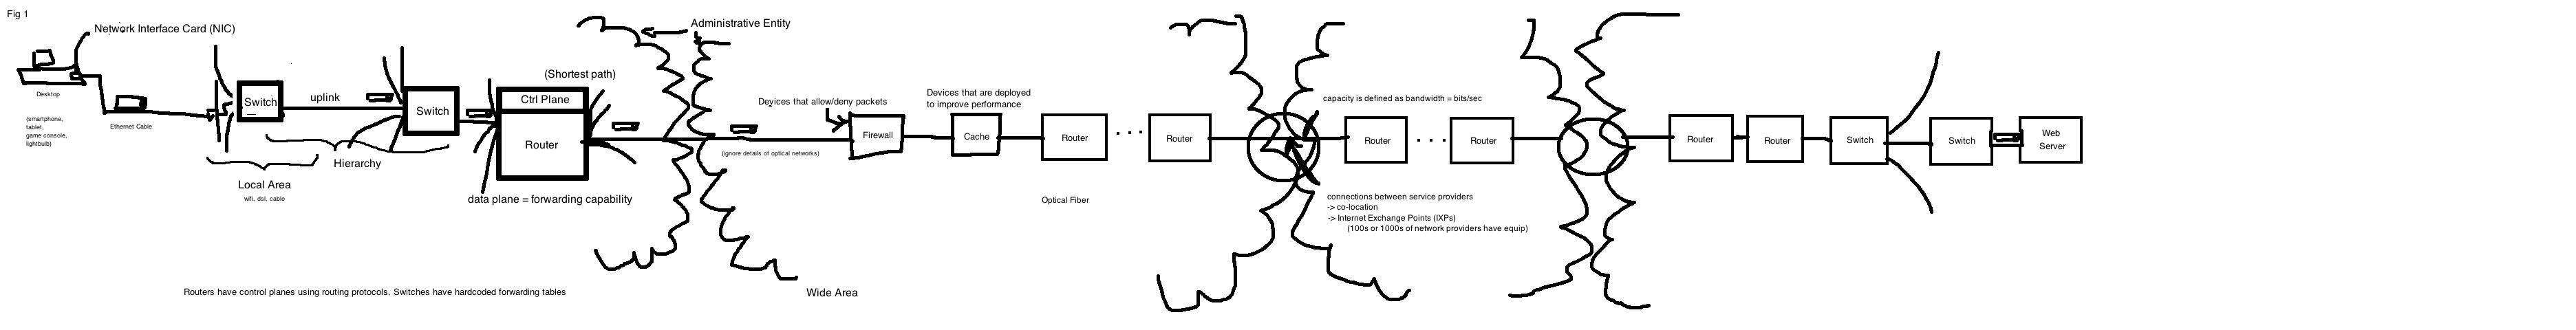
\includegraphics[width=.9\linewidth]{diagrams/fig1.png}

\begin{itemize}
\item Service providers run network administrative domains and are
defined in tiers:
\end{itemize}
Tier 1) Very large providers with world wide footprint (ie AT\&T)
Tier 2) Single entities or providers with a more restricted
infrastructure (ie IBM, Microsoft)
Tier 3) Local service providers

\subsection{Architectural Perspective}
\label{sec:orgheadline8}
\begin{itemize}
\item Guide for implementation
\begin{itemize}
\item Model for reasoning about complex systems
\begin{itemize}
\item Primary abstraction = layers
\end{itemize}
ex of layered architecture)
\end{itemize}
\end{itemize}
\begin{verbatim}
       |-+|
       | garments    |                                                                            |
       | cloth       | - Stack: we move up by providing increased levels of service at each layer |
       | yarn/thread |                                                                            |
       | fibers      |                                                                            |
       |-+|
\end{verbatim}

\begin{itemize}
\item Abstract layered architecture for network:
\end{itemize}
\begin{center}
\begin{tabular}{l}
+\\
applications & <- Actual programs that facilitate communication\\
process-to-process & <- Multiplexing hosts and addressing reliability\\
host-to-host & <- Abstracts network complexities between hosts\\
hardware & <- Actual connections\\
+\\
\end{tabular}
\end{center}

\section{9/19/17  Architectural Perspective / Performance}
\label{sec:orgheadline20}

\subsection{Primary abstraction = Layers}
\label{sec:orgheadline10}
\begin{itemize}
\item Decompose complexity into manageable chunks
\item Increased levels of 'service' as we move from bottom to top
\item Protocols are defined at each layer
\begin{itemize}
\item Protocols provide services for higher layers to communicate
\end{itemize}
\item Set of layers that define the system/internet = \textbf{stack}
\end{itemize}

\subsection{Protocols}
\label{sec:orgheadline15}
\begin{itemize}
\item Define 2 interfaces:
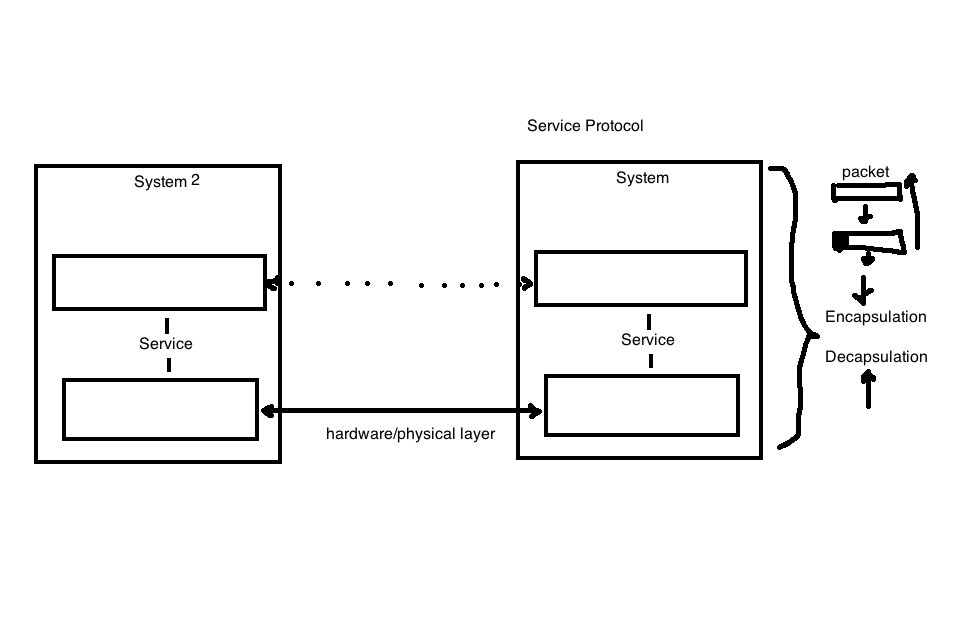
\includegraphics[width=.9\linewidth]{diagrams/fig2.png}
\begin{enumerate}
\item \textbf{Service}: Defines local operations that can be performed - interface
that can be performed - interface between layers on same system
\item \textbf{Peer}: Defines the form/meaning of messages exchanged between the same
protocol layer on 2 different systems
\end{enumerate}
\end{itemize}

\subsubsection{Notes:}
\label{sec:orgheadline11}
\begin{itemize}
\item Bits are only actually exchanged by hardware (at the hardware level)
\item Potentially multiple protocols defined at each layer
\item \emph{NTP is a read-able RFC}
\item Protocol is an overloaded term:
\begin{itemize}
\item Description of how something behaves
\item Algorithms or state machine
\item Definitions
\end{itemize}
\end{itemize}

\subsubsection{First Internet Architecture (OSI model)}
\label{sec:orgheadline12}
\begin{itemize}
\item Defined by ISO
\item Open Systems Interconnection model (OSI), 7 layers
\end{itemize}

\subsubsection{Internet Architecture}
\label{sec:orgheadline14}
\begin{itemize}
\item \textbf{5 layer model}:
\end{itemize}
\begin{center}
\begin{tabular}{l}
\sout{-}-\\
Layer & Name & Description\\
\sout{-}-\\
L5 & Application & Defines interactions with users, and when to initiate/receive transfers\\
OSIs have additional layers here &  & \\
L4 & Transport & Defines logical channels between network and applications\\
L3 & Network & Defines addressing and routing (ie IP)\\
L2 & Link & Defines how hosts access physical media (ie Ethernet)\\
L1 & Physical & Defines media, physical layout, and how bits are represented\\
\sout{-}-\\
\end{tabular}
\end{center}
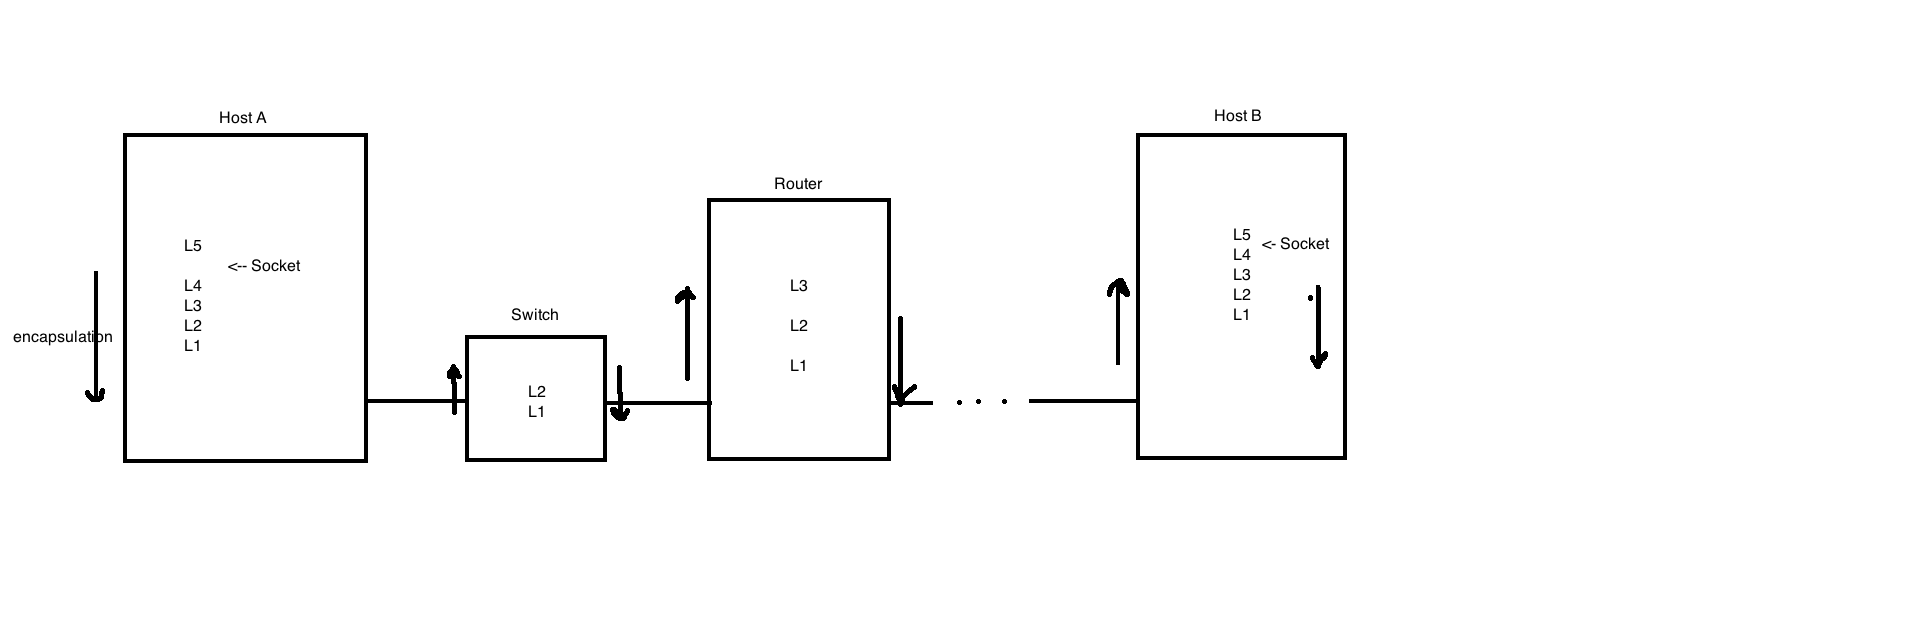
\includegraphics[width=.9\linewidth]{diagrams/fig3.png}

\begin{itemize}
\item Layer 3 has one protocol = \textbf{Internet protocol (IP)}
      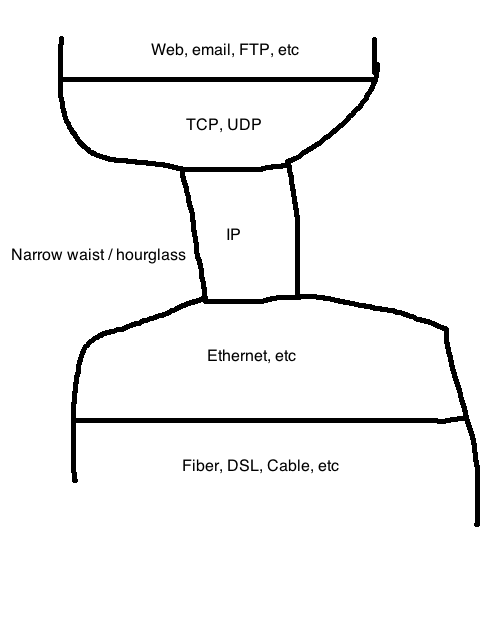
\includegraphics[width=.9\linewidth]{diagrams/fig4.png}

\item In practice, implementations don't necessarily respect layers
\end{itemize}

\begin{enumerate}
\item \textbf{IP Service Model}
\label{sec:orgheadline13}
\begin{itemize}
\item Will be quizzed/tested on this
\item Gives us destination-based forwarding:
\begin{enumerate}
\item Connectionless
\item Packet-based
\item Best effort: packets can be delayed, dropped, reordered, or duplicated
\end{enumerate}
\end{itemize}
\end{enumerate}

\subsection{Performance}
\label{sec:orgheadline18}
\begin{itemize}
\item \emph{The ability to make communication faster} -> has been a major driver of
Internet technology
\end{itemize}

\subsubsection{Basics:}
\label{sec:orgheadline17}
\begin{itemize}
\item \textbf{Bandwidth}: The amount of data that can be transferred per unit of time
\end{itemize}

\begin{enumerate}
\item Link vs End-to-End:
\label{sec:orgheadline16}
\begin{itemize}
\item Link = source to destination (basically bandwidth).
\item End to end = notion that there are destinations inbetween source \&
destination
\begin{itemize}
\item Performance can be defined in terms of \textbf{Latency} (time to send message
from one host to another)

\emph{Latency = Propogation + Queuing + Transmit}
Propogation delay \textasciitilde{}= distance / speed of light
Queuing delay = [0\ldots{}Queue1+Q2\ldots{}Qn | n = number of hops]
Transmit delay = Amount of data to send / Bandwidth

\begin{itemize}
\item Propogation Delay * Bandwidth = amount of data 'in flight' or 'in
the pipe' = \textbf{delay, bandwidth product}
\end{itemize}
\end{itemize}
\end{itemize}
\end{enumerate}
\subsection{HW1}
\label{sec:orgheadline19}

\section{9/26/17  Information Theory Basics / Simple Reliability / Physical Layer}
\label{sec:orgheadline28}

\begin{itemize}
\item Review: IP enables communications between networks
\item Encapsulation as packet moves down, decapsulation as packets move up the
stack \textbf{headers}
\item \textbf{Scalability, Robustness, Performance}
\end{itemize}

\subsection{Queuing}
\label{sec:orgheadline21}

\emph{Latency = Propogation + Queuing + Transmit}
\begin{itemize}
\item Queuing Models and Analysis is a huge area of study
\item Basic Queue:

input->[Buffer](Server)->output 
\^{} packet processes

\begin{itemize}
\item Buffer manangement policies (ie. FCFS, LCFS, priority)
\item Server: \# and speed
\item Server Delay = outgoing bandwidth
\item \textbf{Little's Law:} Mean \# of jobs in system = arrival rate * mean response
time
\emph{arriving jobs -> [black box] -> departing jobs}

\begin{itemize}
\item Applies when jobs entering = jobs leaving (no jobs are dropped or created)
\item ex) Avg forwarding time in a router is 100 nanoseconds. The I/O rate =
100k pps. What is the mean \# pkts in buffer? Solution: Mean \# packers
in buffer = 100,000 * 0.0001 = \textbf{10}
\end{itemize}
\end{itemize}
\end{itemize}

\subsection{Information Theory Basics}
\label{sec:orgheadline26}

1700s: G. Boole invents Boolean Logic
\begin{itemize}
\item AND/OR/NOT, 0, 1

Problem: Transmission of information over a \textbf{noisy channel}
Objective: Reproduce a message at some point that was sent at another point
\end{itemize}

\subsubsection{C. Shannon: 1948: "A Mathematical Theory of Communication"}
\label{sec:orgheadline23}
-> foundation for Information Theory
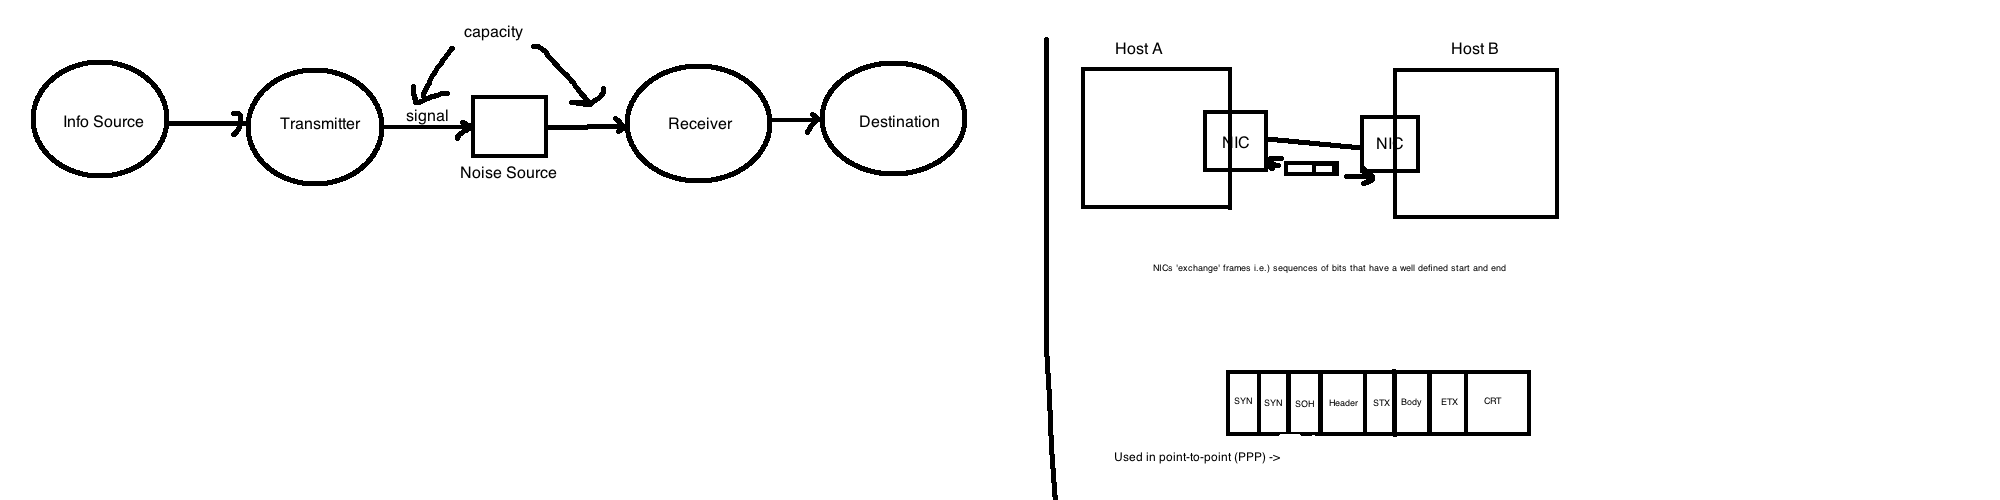
\includegraphics[width=.9\linewidth]{diagrams/fig5.png}

\uline{Definitions:}
\textbf{Information} (measured in bits): The amount of uncertainty a message
eliminates or only \uline{\_\_} uncertain to a receiver
\textbf{Noise} distorts a message. Reduces information by increasing uncertainty
\textbf{Redundancy:} Repetition of a message or part of a message that reduces information loss due to noise
\textbf{Channel Capacity:} Amount of information + noise that can be processed per
unit of time

\begin{enumerate}
\item Key Results:
\label{sec:orgheadline22}
\begin{enumerate}
\item Quantifies the average number of bits needed for communication in terms
of \textbf{entropy} (quantifies uncertainty) -> \textbf{source coding theorem}
\item Proves that reliable communication is possible over a noisy channel if
\emph{transmit rate < capacity} -> \textbf{noisy channel coding theorem}
\end{enumerate}
\end{enumerate}

\subsubsection{Handling Errors/Noise}
\label{sec:orgheadline25}
\begin{itemize}
\item We should drop packets with errors as soon as possible
\uline{Reasons}
\begin{enumerate}
\item Not useful for apps that assume reliable transfer
\item Saves resources downstream
\end{enumerate}
\end{itemize}

\begin{enumerate}
\item How do you know that a packet has an error?
\label{sec:orgheadline24}
(at least one bit is flipped)
\begin{enumerate}
\item Packet = Datagram D = string of bits
\item Use algorithm A on D to generate code C = string of bits
\item Transmit D,C
\item Receiver gets D,C, uses Algorithm A on D to get C' and compares C and C'

\item The \textbf{expected noise} determiens the type of encoding that is required. 

\uline{Typical Methods of Encoding}
\begin{enumerate}
\item \textbf{Parity:} odd/even, 1-bit code
\item Checksum
\item \textbf{Cyclic Redundancy Check (CRC)} Need to know algorithm! Look it up
in the book
\begin{itemize}
\item Modular arithmetic
\end{itemize}
\end{enumerate}

\item Error checking is done at almost ever layer in the protocol stack
\end{enumerate}
\end{enumerate}

\subsection{Layer 1: Physical Layer}
\label{sec:orgheadline27}

\uline{Concerned with:}
\begin{enumerate}
\item Characteristics of hardware and physical media
\item Signals on physical media, and framing -> where packets begin and end on
physical media
\item Framing - where packets begin and end on physical media

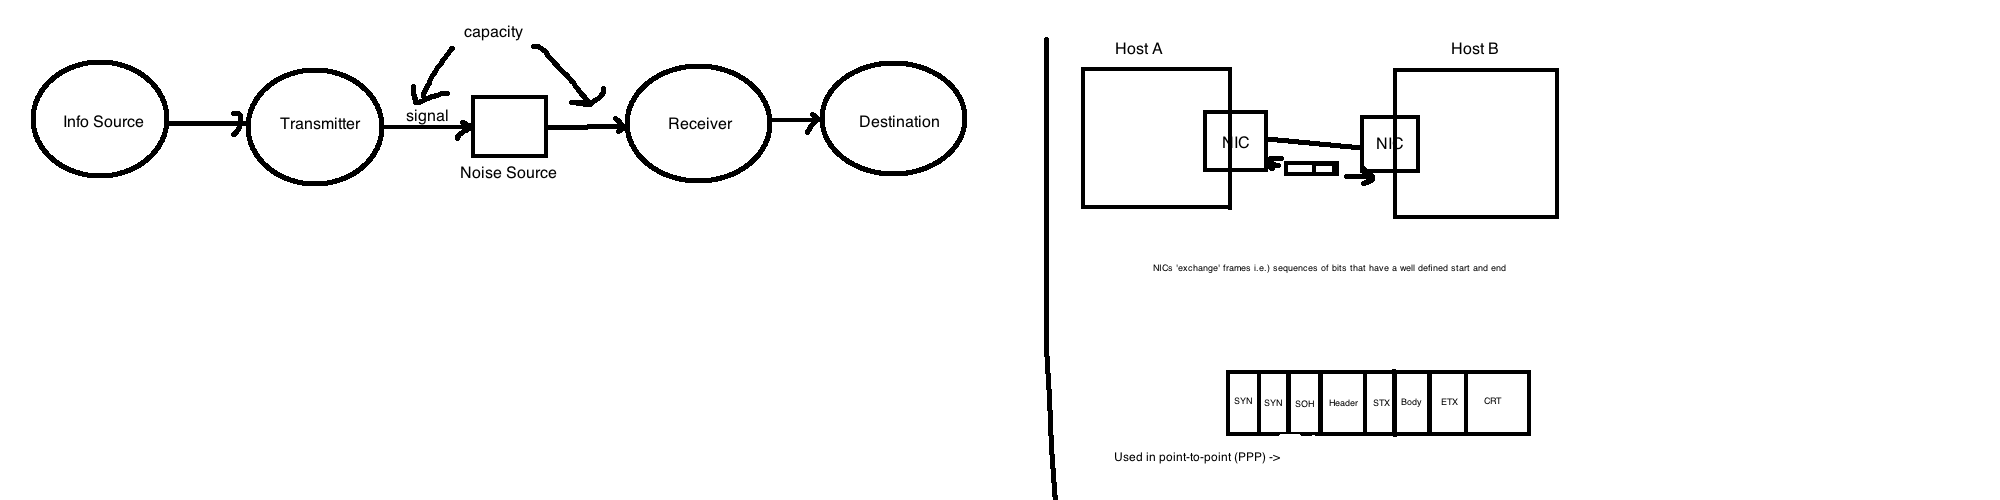
\includegraphics[width=.9\linewidth]{diagrams/fig5.png}
\begin{itemize}
\item NICs 'exchange' frames ie) sequences of bits that have a well defined
start and end
\item How are start and end identified?
\begin{enumerate}
\item \textbf{Sentinel Approach}: Uses special characters to delineate start and
end. SYN, STX, ETX
\item Byte Counting
\item Clock-based
\end{enumerate}
\end{itemize}
\end{enumerate}

\section{9/28/17  Framing}
\label{sec:orgheadline30}
\subsection{Layer 1 Continued}
\label{sec:orgheadline29}

\uline{Framing}:
\begin{enumerate}
\item Sentinal:
\end{enumerate}

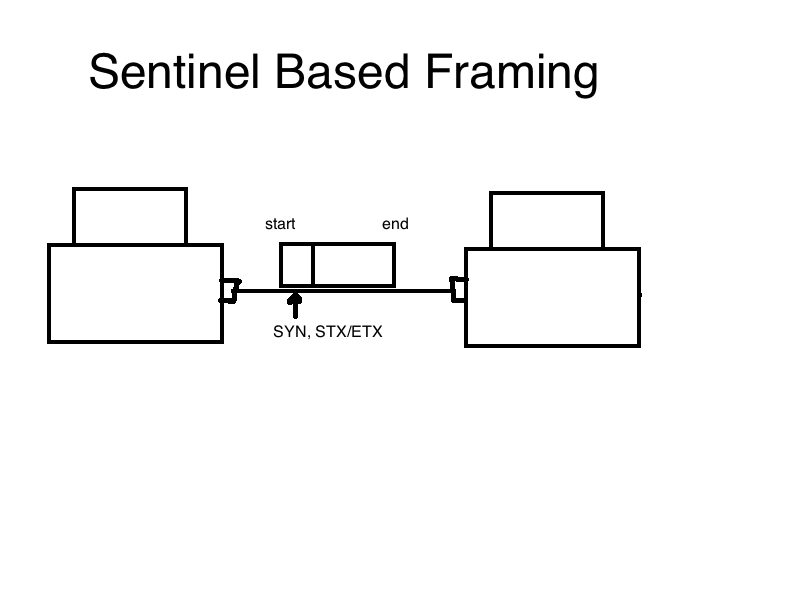
\includegraphics[width=.9\linewidth]{diagrams/fig6.png}

\begin{enumerate}
\item Byte counting - SYN + \#Bytes
\item Clock-based:
\begin{itemize}
\item Fixed frame size
\item Includes special characters
\item Need to use timing to determine the start and end
\end{itemize}
\end{enumerate}

Aspects that are included:
\begin{itemize}
\item Details of hardware (connectors, cables, etc)
\begin{itemize}
\item Coax, Twisted pair, \textbf{Optical Fiber}
\end{itemize}
\item Transmission of bits between hosts. That is how to represent 1s and 0s

\item Transmission medium = copper
\begin{itemize}
\item Transponder modulates voltage
\begin{itemize}
\item 0 = no voltage
\item 1 = voltage
\emph{How are multiple 1s and 0s distinguished?}
Solution = clock

\emph{Non-Return to Zero (NRZ):} 0 = low, 1 = high voltage
\begin{itemize}
\item Requires clock synchronization
\item Keep an average voltage to distinguish high and low
\end{itemize}
\emph{NRZ-Inverted (NRZI):} 0 = staying at same signal, 1 = changing signal
\emph{Manchester Encoding:} Explicit merge of clock and data, encode both 0
and 1 as transitions
\begin{itemize}
\item 1 = high-to-low transition
\item 2 = low-to-high transition
\item Move back to baseline as needed inbetween clock edges
\end{itemize}
\end{itemize}
\end{itemize}
\end{itemize}

\section{10/3/17  Data Link (Layer 2)}
\label{sec:orgheadline38}

\subsection{Project 1}
\label{sec:orgheadline31}
\begin{itemize}
\item In the \emph{Switchyard environment} -> enables switches, routers, etc to be built/emulated
\begin{itemize}
\item Focused on sending / receiving / processing and forwarding packets
\end{itemize}

\item Install VM on Linux-based system (see project homepage)
\begin{itemize}
\item Switchyard + Mininet
\end{itemize}
\item Do learning-switch exercise (.rst)
\begin{itemize}
\item see detail on Project 1 page
\end{itemize}
\item Submit program files by deadline (10/19)
\item Grading:
25\% = code review
25\% = code does minimal subset of functions
25\% = code runs correctly
25\% = answering a set of questions that can be answered once the code runs
\end{itemize}

\subsection{Layer 2 - Data Link}
\label{sec:orgheadline32}
Concerned with transfer of data between adjacent hosts. Hosts are within same
"local area" -> several hundred meters. There are 3 different types of
channels between hosts.

\begin{enumerate}
\item \textbf{Point-to-Point}
\begin{itemize}
\item Single or full duplex
\item Framing
\item Reliability
\end{itemize}
\item \textbf{Broadcast} = enable more systems to communicate
\begin{itemize}
\item Challenge -> coordinating between hosts
\begin{itemize}
\item Media Access Control protocol (MAC)
\item Include additional specifications and addressing schemes
\end{itemize}
\end{itemize}
\item \textbf{Switched}
\end{enumerate}

\subsection{MAC (Media Access Control)}
\label{sec:orgheadline34}
\begin{enumerate}
\item Channel Partitioning
\begin{itemize}
\item Time division multiplexing
\item Frequency division multiplexing
\item Code division multiplexing
\end{itemize}

\item Taking turns
\begin{itemize}
\item Polling
\item Token passing
\end{itemize}
\end{enumerate}

\subsubsection{3. Random Access}
\label{sec:orgheadline33}
\begin{itemize}
\item Nodes send/receive in no specific order
\item Challenge: managing contention (ie. when two or more nodes want to send at
the same time)
\end{itemize}

\subsection{Aloha Network}
\label{sec:orgheadline35}
Packet radio in late 60s / early 70s
\begin{itemize}
\item Send immediately
\item Receivers will send an ACK
\item If sender hears that another node is transmitting, then rest and resend
(since original was assumed lost)
\item If sender does not receive ACK within some time period, rest and resend
\item Solves contention, but is inefficient
\end{itemize}

\subsection{Ethernet}
\label{sec:orgheadline37}
\begin{itemize}
\item Invented by Metcalf -> '73
\item Spans layer 1 \& 2
\item Bus-based
\begin{itemize}
\item Also hubs
\item Bridged Environments
\item Switched (Provides virtual point-to-point communication channels)
\end{itemize}
\end{itemize}

\subsubsection{Ethernet Frames}
\label{sec:orgheadline36}
\begin{itemize}
\item Well defined
\item Include:
\begin{enumerate}
\item Preamble
\item Src/Dst addresses (48 bits)
\item Payload
\item Flags
\item CRC Checksum
\end{enumerate}
\item Service: Connectionless and unreliable
\end{itemize}

\section{10/5/17  Ethernet MAC, Interconnects}
\label{sec:orgheadline45}

\subsection{Ethernet}
\label{sec:orgheadline42}

\subsubsection{802.3 ethernet protocol}
\label{sec:orgheadline39}
\^{} wire-line ethernet \emph{on quiz/exam!!}
\begin{itemize}
\item 10Mbps -> ie) it takes 0.1 \(\mu\) s to signal 1 bit
\end{itemize}
\begin{itemize}
\item \textbf{MAC} = carrier sense multiple access colision detect (CSMA/CD)
\begin{enumerate}
\item If the line is idle, send immediately, then wait for 9.6 \(\mu\) s between
frames (interframe gap)
\item If line is busy, wait until it's clear + 9.6 \(\mu\) s
\item If a collision is detected, send jam signal (32-48bits), do \emph{exponential
backoff}
\begin{itemize}
\item purpose of jamming signal is to ensure/reinforce that all nodes know
there was a collision

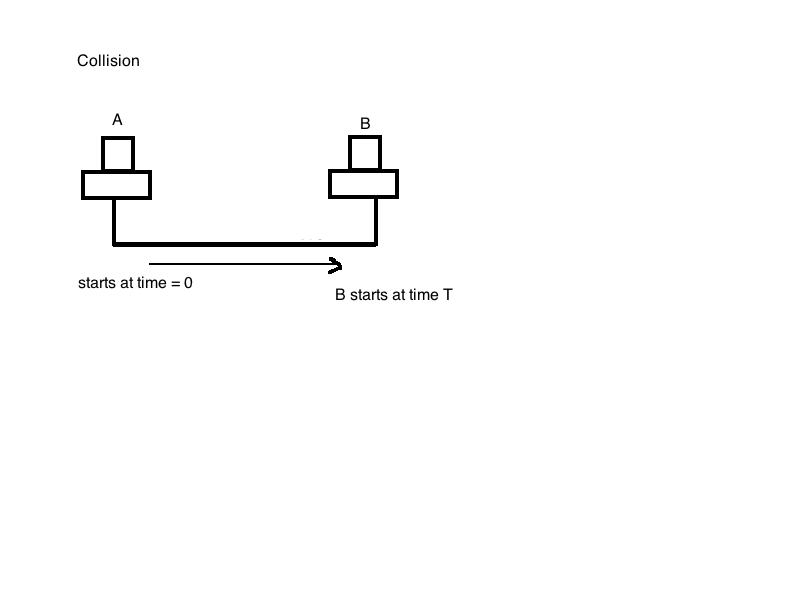
\includegraphics[width=.9\linewidth]{diagrams/fig7.png}
\end{itemize}
\^{} Problem: ensuring the A sees collision
B's message gets to A at time = 2T
Solution: Be sure that A is still transmitting at time = 2T
\end{enumerate}

\item 802.3 specifies that 2Tmax = 51.2 \(\mu\) s
\begin{itemize}
\item Thus at 10Mbps this means min frame size = 512 bits (64B)
\item This also implies max length of an Ethernet bus segment = \textasciitilde{}2500m
\item Frame header = 18B
\item If data < 46B, add padding
\end{itemize}

\item Collision domain = CSMA/CD network where there will be a collision if 2
nodes transmit at the same time
\end{itemize}

\subsubsection{Exponential backoff}
\label{sec:orgheadline40}
1st collision: chose k from \{0,1\} then delay k*57.2 \(\mu\) s
2nd collision: chose k from \{0,1,2,3\} then delay k*57.2 \(\mu\) s
\ldots{}
10th collision: max -> notify the higher layers that was unable to send frame

\subsubsection{Ethernet efficiency}
\label{sec:orgheadline41}
\textasciitilde{} $\backslash$(1/1+(5*tprop)/ttrans))
\begin{itemize}
\item larger frame in smaller network = more efficient network

\begin{itemize}
\item \emph{Quiz question}: how do things change if we move from 10Mbps to 100 Mbps
\end{itemize}
\end{itemize}


\subsection{Ethernet Interconnects}
\label{sec:orgheadline44}
Problem: How do we extend or interconnect Ethernet segments?

\subsubsection{Interconnection devices}
\label{sec:orgheadline43}
\begin{enumerate}
\item \textbf{Hub} - most simple ethernet interconnect which \emph{does not} extend the
collision domain
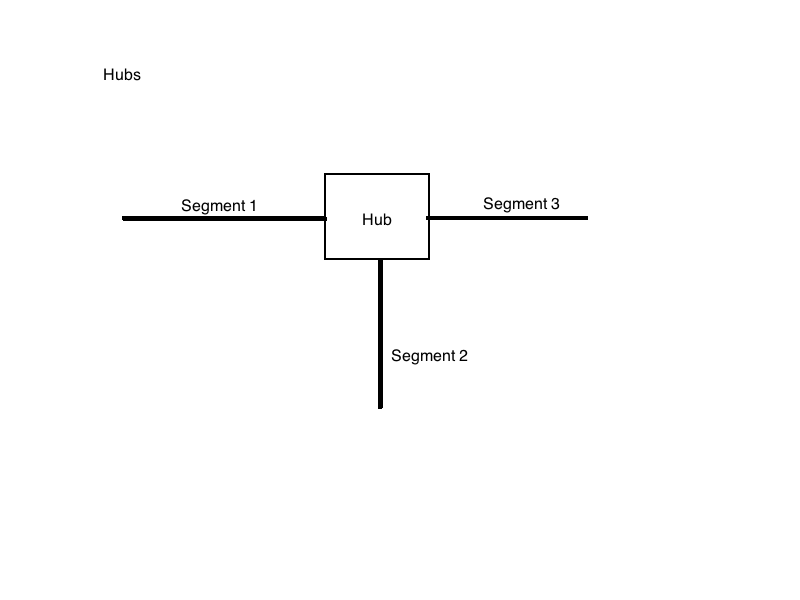
\includegraphics[width=.9\linewidth]{diagrams/fig8.png}
\item \textbf{Bridge} - device that connects together 2 different collision domains
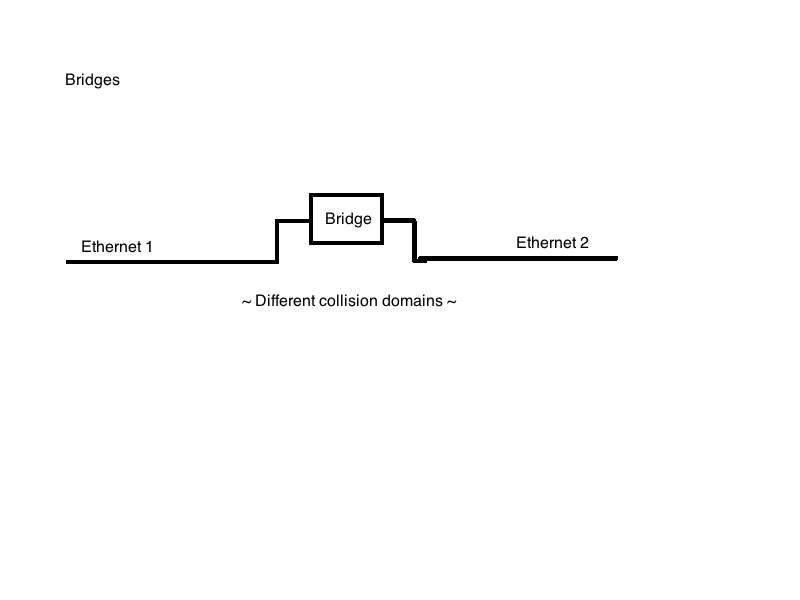
\includegraphics[width=.9\linewidth]{diagrams/bridge.png}
\begin{itemize}
\item Collision domains are separate, bridges forward frames based on
destination addresses
\begin{itemize}
\item Bridges build forwarding tables or through fixed configuration
\end{itemize}
\item Bridgin can enable larger LANs. However, managing large LANs depends on
another protocol -> \textbf{Spanning Tree} which organizes LANS in a tree that
assures a loop-free hierarchy
\item Makes forwaring decisions based on Ethernet / MAC addresses
\end{itemize}
\end{enumerate}

\section{10/10/17  Switching, Wifi, Layer 3}
\label{sec:orgheadline53}

\subsection{Ethernet Switches}
\label{sec:orgheadline46}
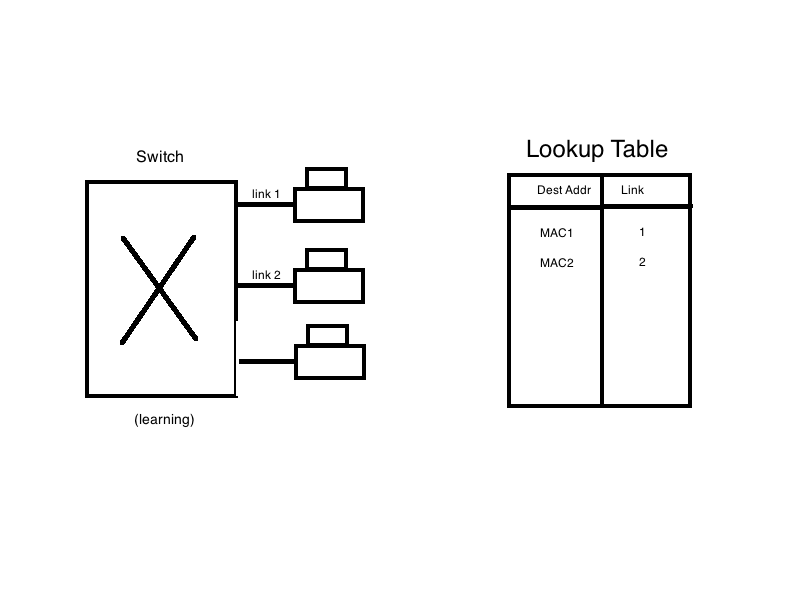
\includegraphics[width=.9\linewidth]{diagrams/switch.png}
\begin{itemize}
\item Overcome the limitation of bus/hub by isolation collision domains to
2 hosts. Forwarding decisions are based on destination MAC addresses
\item Basic function is to lookup destination address in a table and
forward packet/frame on associated link/segment
\item Switches build tables automatically:
\begin{enumerate}
\item Empty Table
\item If dest. addr. is NOT in table, forward frame on all links
(except for the link that sent frame)
\item When a frame arrives with source address that's not in the table,
create new entry for addr/link
\item Delete table entry if no frame is received from source after some
timeout period
\end{enumerate}
\end{itemize}

\subsection{Wireless LANs}
\label{sec:orgheadline51}
\begin{itemize}
\item Transmit / Receive data via antennas
\item \textbf{802.11} = Set of standards for wireless LANs
\item Wireless networks are different:
\begin{itemize}
\item It's hard to transmit and listen at the same time -> due to
antennas
\item Carrier sense is weaker
\item The air is not a perfect broadcast environment
\end{itemize}
\end{itemize}
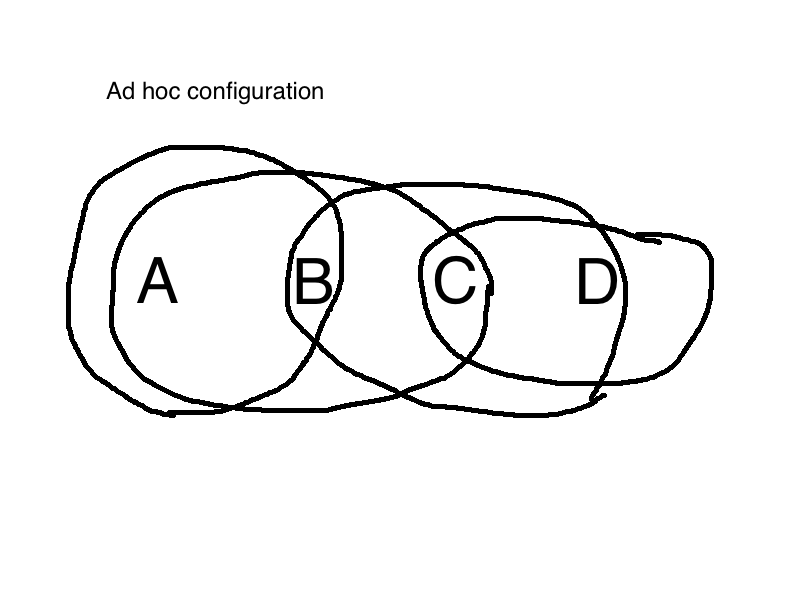
\includegraphics[width=.9\linewidth]{diagrams/adhocconfig.png}
\begin{itemize}
\item When B transmits, A and C can hear
\item When A or C transmits, B can hear
\end{itemize}

\subsubsection{Problems}
\label{sec:orgheadline47}
\begin{itemize}
\item If A transmits to B, C cannot hear, so it will send to B at any time
\begin{itemize}
\item This can corrupt the message A is sending = \textbf{The hidden terminal
problem}
\end{itemize}
\item If B is sending to A, C can hear it so it won't transmit. But, it
could send to D since this transmission would not interfere with A's
reception = \textbf{The exposed terminal problem}
\item These problems are particular to carrier sense wireless ad hoc LAN
\end{itemize}

\subsubsection{Solution: Multiple Access with Collision Avoidance (MACA) protocol*}
\label{sec:orgheadline48}
\begin{itemize}
\item Solution to these problems
\item Basically a connection setup protocol
\begin{enumerate}
\item Before sending data, a sender transmits \textbf{Request to Send (RTS)}
     frame that includes a duration
\item Receiver sends \textbf{Clear to Send (CTS)} that echos the duration
\item Receiver sends ACK on successful receipt of frame, other nodes
wait for this
\end{enumerate}
\item The CTS solves hidden terminal by informing nodes within range of
the receiver how long they need to be quiet
\item Any node that receives RTS but does not receive CTS knows that they
are not close enough to the receiver to interfere -> solves exposed
terminal
\end{itemize}
\textbf{If there is a collision on FTS due to carrier sense, do random
exponential backoff} 

\subsubsection{Access Points}
\label{sec:orgheadline50}
\begin{itemize}
\item Today's WiFi(802.11) LANs are facilitated through access points
(APs) that acts as \textbf{switches}. APs in a local area are connected via
wireline Ethernet
\end{itemize}
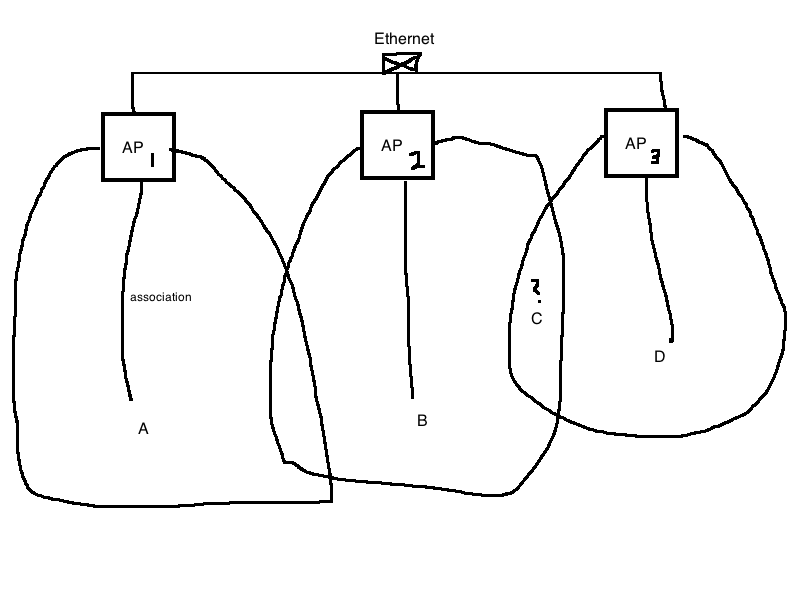
\includegraphics[width=.9\linewidth]{diagrams/accesspoint.png}
\begin{enumerate}
\item Association Protocol
\label{sec:orgheadline49}
\begin{enumerate}
\item WiFi node scan for access points by sending probe frame
\item All APs that receive probe frames send Probe Response Frame
\item Node selects AP with the strongest signal and sends Association
Request Frame
\item AP responses with Association Response frame
\end{enumerate}
\end{enumerate}

\subsection{Layer 3 - Network Layer}
\label{sec:orgheadline52}
\begin{itemize}
\item One of the most important aspects of Layer 3 - the one that makes it
the narrow waist - is the unified addressing scheme (ie \textbf{Internet
Protocol Addresses})
\end{itemize}

\section{10/12/17  Network Layer 3}
\label{sec:orgheadline60}
\begin{itemize}
\item Addressing - Single scheme
\item Routing protocols
\item Routers
\item \textbf{Major layer 3 activity}: move packets between networks
\end{itemize}

\subsection{Layer 3 Architecture}
\label{sec:orgheadline54}
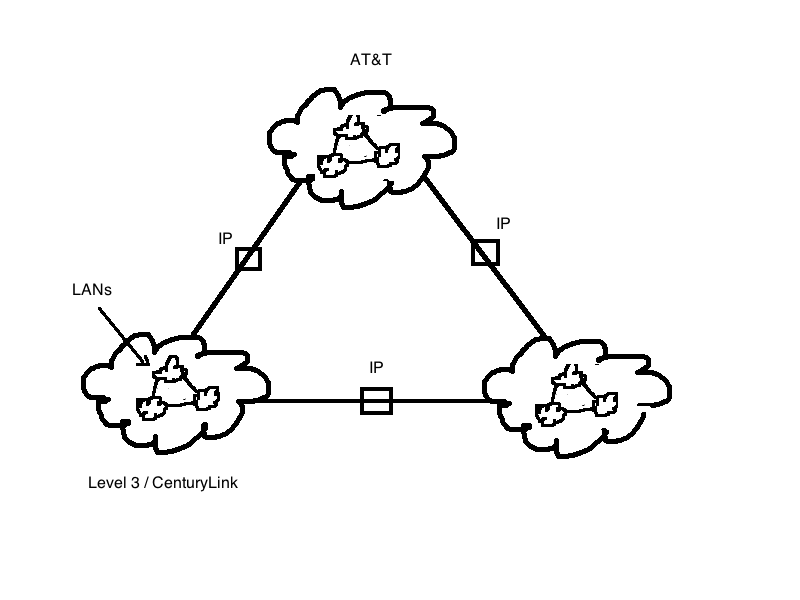
\includegraphics[width=.9\linewidth]{diagrams/layer3.png}
\begin{itemize}
\item Autonomous System (AS) = Independent administrative domain <- ISPs
\end{itemize}

\subsection{IP Addresses (IANA)}
\label{sec:orgheadline59}
\begin{itemize}
\item 32-bit numbers organized in \emph{dot notation}
\begin{itemize}
\item ie: 192.128.65.80, each dot seperates 8 bit portion
\item 4 billion possible addresses
\item IPv4
\end{itemize}
\end{itemize}

\subsubsection{Address allocation}
\label{sec:orgheadline55}
\begin{itemize}
\item Address allocation to networks is a very big deal
\begin{itemize}
\item Networks are defined by their address space
\end{itemize}
\item Original IPv4 address space allocation was "classful"
\end{itemize}

\begin{center}
\begin{tabular}{ll}
\hline
Class & Address Space\\
\hline
A & [0(1bit),Network(7bit),Host(24bit)]\\
B & [1(1bit),0(1bit),Network(14bit),Host(16bit)]\\
C & [1(1bit),1(1bit),0(1bit),Network(21bit),Host(8bit)]\\
D & 110\ldots{}Multicast\\
E & 1111\ldots{}Experimental\\
\hline
\end{tabular}
\end{center}

\begin{itemize}
\item Routers examine the network portion of addresses to make forwarding
decisions
\item Classful allocation presents a number of scalability challenges:
\begin{itemize}
\item Inflexible
\item Too many networks
\item Plus, we may not be able to manage large networks on Layer 2 by
itself
\end{itemize}
\end{itemize}

\subsubsection{Subnets}
\label{sec:orgheadline56}
\begin{itemize}
\item Enables a single allocation of IP addresses to be divided into
smaller 'networks'
\begin{itemize}
\item Allows us to do routing using layer 3 packet forwarding in an
administrative domain
\end{itemize}
\item Subnets arrange for an extension into the host portion of an
address:
\end{itemize}

\begin{verbatim}

 16bit  16bit      16bit      8bit      8bit
[ Net ][ Host ] -> [ Net ][ Subnet ID ][ Host ]
                       net + subnet ID = subnet number
\end{verbatim}

\begin{itemize}
\item Subnets are identified by bitwise AND of IP address and the \textbf{Subnet
mask}
\begin{itemize}
\item Ex. 255.255.255.0 would expose the subnet in the prior example
\item This means that forwarding table must include subnet masks
Forwarding table entries: < subnet number, subnet mask, link >
\end{itemize}
\end{itemize}

\subsubsection{Supernetting}
\label{sec:orgheadline57}
\begin{itemize}
\item Goal: more flexibility in address space allocation. Supernet says
allocate address space on powers of 2. Classless Interdomain
Routing Addresses (\textbf{CIDR addresses})
\item CIDR indicates network addresses using "/" 
\begin{itemize}
\item ie) 
class C = /24
class B = /16
class A = /8
\end{itemize}
\item CIDR is used in forwarding tables by allowing for adjacent networks
to be "combined"
\end{itemize}
\begin{center}
\begin{tabular}{ll}
\hline
Net & Link\\
\hline
Class B1 & Link A\\
Class B2 & Link A\\
\hline
\end{tabular}
\end{center}

goes to\ldots{}

\begin{center}
\begin{tabular}{ll}
\hline
/15 & Link A\\
\hline
\end{tabular}
\end{center}

\textbf{ON QUIZ}
How do packets get to hosts?
Answer: build a table that maps IP addresses to MAC addresses
associated with hosts.

\subsubsection{Address Resolution Protocol (ARP)}
\label{sec:orgheadline58}
\begin{itemize}
\item A dynamic protocol that operates by:
\begin{enumerate}
\item Switch begins by looking for entry in table (IP address / MAC)
\item Broadcast request over a LAN
\item Node with IP address responds with ARP\(_{\text{response}}\)
\item Each entry has a time to live
\end{enumerate}
\end{itemize}

\section{10/17/17  DHCP, Routers, Routing}
\label{sec:orgheadline67}

\subsection{Dynamic Host Control Protocol (DHCP)}
\label{sec:orgheadline61}
\begin{itemize}
\item Enables hosts to have an address assigned for the local network
\item Hosts send a special address request packet to address
255.255.255.255 and listens for a response at layer 2. Response
comes from local DHCP server
\end{itemize}

\subsection{Router Design}
\label{sec:orgheadline62}
\begin{itemize}
\item Routers operate at layers 1-3 of the protocol stack. Physical
hardware that ranges from low-cost home devices to "core systems"
that cost \$\$\$. The primary task of routers is to make
(destination-based) forwarding decisions - using destination IP
addresses <- network portion or subnet
\item The other task of routers is to participate in \textbf{routing protocols}
  that establish local \emph{fowarding tables} (unlike switches which use learning)
\end{itemize}

\subsection{Router Types}
\label{sec:orgheadline63}
\textbf{Simple Routers:}
\begin{itemize}
\item Single board (running linux)
\begin{center}
\begin{tabular}{l}
[]  [][][][]\\
\end{tabular}
\end{center}
\item Uplink + 4 local ethernet ports / 1Gbps
\item Limited management/config
\item Limited protocol support
\item Low cost
\end{itemize}

\textbf{Access/Distribution Routers:}
\begin{itemize}
\item Single board (often linux)
\item Stackable/rack mount devices
\end{itemize}
\begin{center}
\begin{tabular}{l}
[-][-][-][-][-][-][-][-][-]\\
\end{tabular}
\end{center}
\begin{itemize}
\item Uplink + 48 ports / 10Gbps
\item Full set of management/config capabilities
\item Moderate cost
\end{itemize}

\textbf{Core/Backbone Routers:}
\begin{itemize}
\item Focus = transmission of large amounts of data over long paths
\item Full or multi-rack systems
\item Specialized ASIC's (application specific integrated circuits)
running proprietary OS's
\item Hundreds of ports/up to \emph{400 Gbps}
\item Hardware layout is focused on reliability and cooling
\end{itemize}
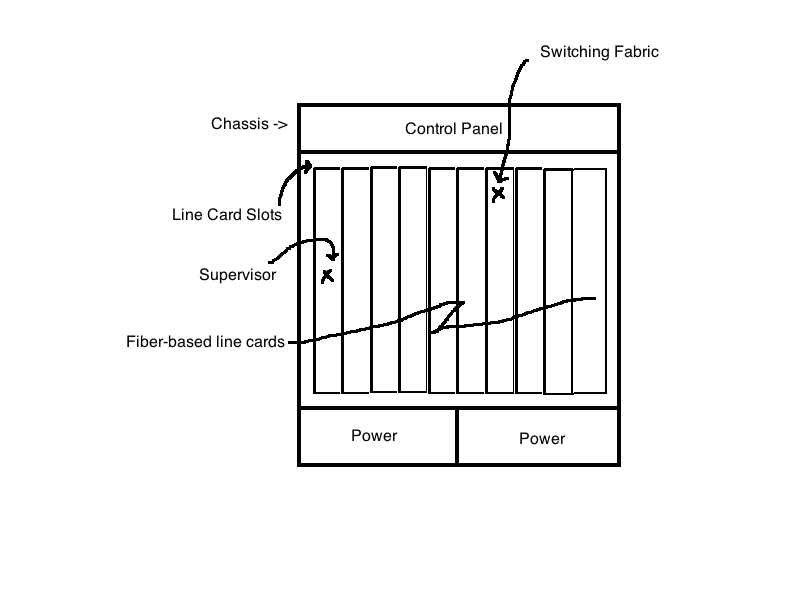
\includegraphics[width=.9\linewidth]{diagrams/corerouter.png} \\
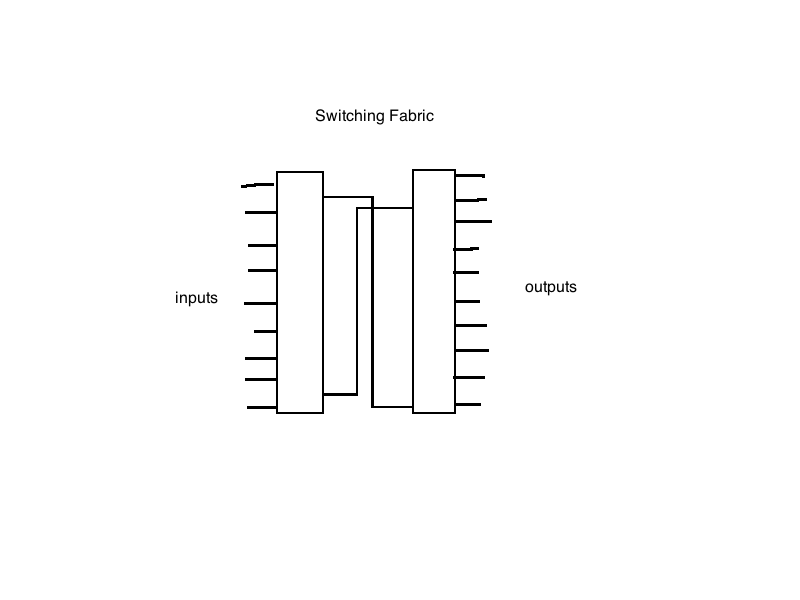
\includegraphics[width=.9\linewidth]{diagrams/switchingfabric.png}

\begin{itemize}
\item Logical organization of routers:
\begin{enumerate}
\item Control plane
\begin{itemize}
\item configs and routing protocols
\end{itemize}
\item Data plane
\begin{itemize}
\item destination-based forwarding
\end{itemize}
\end{enumerate}
\end{itemize}

\subsection{Layer 3 Functions (cont)}
\label{sec:orgheadline66}
Include:
\begin{itemize}
\item Specifying IP packet format
\item Fragmentation / reassembly
\item Error reporting
\item Routing to establish forwarding tables
\end{itemize}

\subsubsection{IP Packet Format}
\label{sec:orgheadline64}
(see fig 3.16 in textbook)
\begin{itemize}
\item Version (4,6)
\item Length of header
\item Type of service
\item Total length (header + payload)
\item \textbf{IPID/flags/offset}
\item TTL (time to live)
\begin{itemize}
\item Each router it encounters decrements the TTL
\end{itemize}
\item Protocol
\item Checksum (header)
\item Src/Dest Addresses
\item Options
\end{itemize}

\subsubsection{Framentation and Reassembly}
\label{sec:orgheadline65}
\begin{itemize}
\item Router designers may select different sizes for pack max size. To
facilitate this, routers should be able to chop up larger packets
into small packets
\item The resulting 'fragments' are identified via IPID and offset
\item Fragmentation is a 'slow-path' process, thus we do MTU \textbf{(Maximum
Transfer Unit)} discovery in TCP
\begin{itemize}
\item If the packet is too large for a router, it sends an error message back
\end{itemize}
\end{itemize}

\section{10/19/17  Routing}
\label{sec:orgheadline76}
Quiz 2 on Tuesday!

\subsection{Internet Control Message Protocol (ICMP)}
\label{sec:orgheadline68}
\begin{itemize}
\item Designed to provide feedback from the network about status
\item 13 message types
\begin{itemize}
\item Ex: TTL = 0, Traceroute
Ex: Echo, Ping
\end{itemize}
\end{itemize}

\subsection{Routing}
\label{sec:orgheadline75}
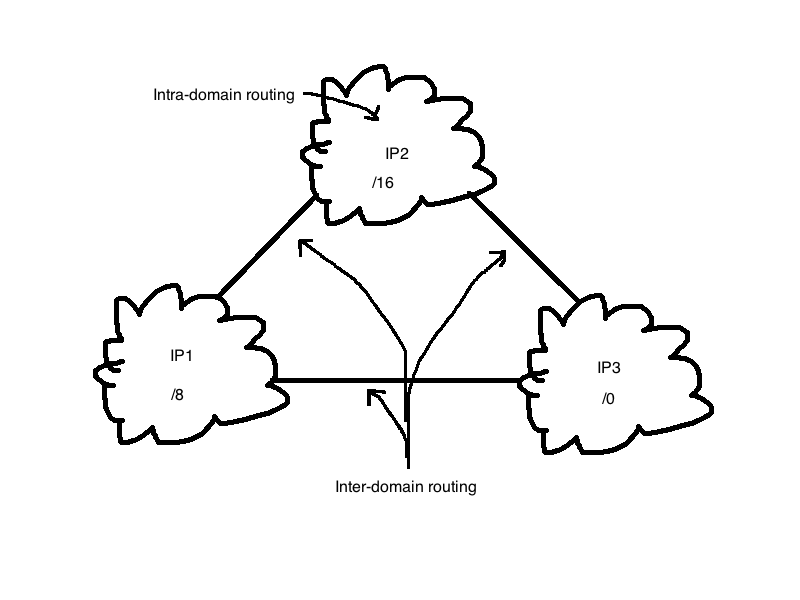
\includegraphics[width=.9\linewidth]{diagrams/routing.png}
\textbf{Routing} = process that is used to establish forwarding tables in
routers.
\subsubsection{2 Levels of Routing}
\label{sec:orgheadline69}
\begin{enumerate}
\item Intra-domain = routing \uline{within} a domain (RIP, OSPF)
\item Inter-domain = routing \uline{between} domains (BGP - don't worry for
quiz 2)
\end{enumerate}

\subsubsection{Intra-Domain Routing}
\label{sec:orgheadline74}

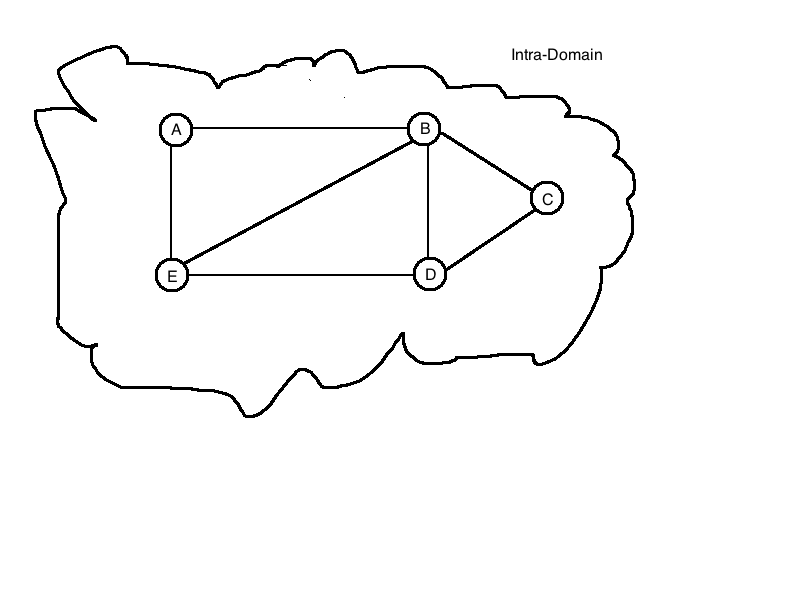
\includegraphics[width=.9\linewidth]{diagrams/intradomainrouting.png}
\uline{Methods for establishing paths:}
\begin{enumerate}
\item Circuit-based (ie telephone)
\item Source-routing
\item Datagram / connectionless
\end{enumerate}

\begin{enumerate}
\item Circuit-based
\label{sec:orgheadline70}
\begin{enumerate}
\item Establish virtual circuits between src and dest prior to sending
data (using signaling protocols)
\item Data and nodes use VC identifiers to forward packets
\end{enumerate}
Pros: Good quality?\\
Cons: Poor utilization?

\item Source routing
\label{sec:orgheadline71}
\begin{itemize}
\item Packets have all info required to move to destination
\item Source must collect hop/path information out of band
\item Each packet has all hops from end-2-end
\end{itemize}
Pros: User control\\
Cons: User control!!

\item Datagram/connectionless
\label{sec:orgheadline72}
\begin{itemize}
\item Each packet is forwarded independently based on destination address
\item Hosts don't know if the destination is reachable
\item Challenge:
\begin{itemize}
\item Find 'lowest-cost' path between source and destination
\item This implies that a cost metric is assigned to each link
\item Easy if network is static, hard in dynamic network (ie the internet)
\end{itemize}
\item This implies the need for an algorithm that establishes shortest
paths quickly and efficiently
\begin{enumerate}
\item Distance Vector Routing
\item Link State Routing: Djikstra's algorithm -> OSPF routing (open
shorest path routing)
\end{enumerate}
\end{itemize}

\item Distance Vector
\label{sec:orgheadline73}
\begin{itemize}
\item Based on local computation by neighbor nodes. Nodes construct and
send 1-d vector of distances to all other nodes
\item Belman-Ford algorithm:
\end{itemize}

\begin{verbatim}
Calculate D[i,j][h] for all i != j
          ^dist  ^hops
h=0, D(i,j)[0] = {0 if i=j, inf otherwise}
h=1, D(i,j)[1] = min/k=neighbors{d(i,k) + D(k,j)) for i != j}
h=2, ^
...
\end{verbatim}

\begin{itemize}
\item Objective is to converge on shortest paths
\item Nodes receive DVs from neighbors periodically or by trigger
\item Everytime a distance vector is received from a neighbor, recalculate
distances
\begin{itemize}
\item This can trigger a forwarding table update
\end{itemize}
\end{itemize}

\emph{Forwarding Table}:
\begin{enumerate}
\item Destination
\item Cost
\item Next Hop (link that packet will be sent out on)
\end{enumerate}

ie)
\begin{center}
\begin{tabular}{lrl}
\hline
Dest & Cost & Next hop\\
\hline
B & 3 & B\\
C & \(\infty\) & -\\
D & \(\infty\) & -\\
E & 1 & E\\
F & 6 & F\\
\hline
\end{tabular}
\end{center}

\begin{itemize}
\item Nodes send DVs to neighbors
\end{itemize}

\begin{verbatim}
if cost neighbor + cost to dest < cost dest:
    update entry for dest
\end{verbatim}

\begin{itemize}
\item \textbf{IMPORTANT} Routing convergence
\end{itemize}
\end{enumerate}

\section{10/24/17  Link State Protocol}
\label{sec:orgheadline84}
\subsection{Cont\ldots{}}
\label{sec:orgheadline77}
\begin{itemize}
\item Distance vectors change because:
\begin{enumerate}
\item A link goes down (edge cost = \(\infty\))
\item A configuration changed
\end{enumerate}

\item Making a link cost low results in more traffic over a particular link
\begin{itemize}
\item ie) A high-bandwidth link can handle more traffic
\end{itemize}
\item Only forward distance vectors when there is a change (or some time
has elapsed)
\end{itemize}

\subsection{Count to Infinity}
\label{sec:orgheadline81}

\subsubsection{The Problem}
\label{sec:orgheadline78}
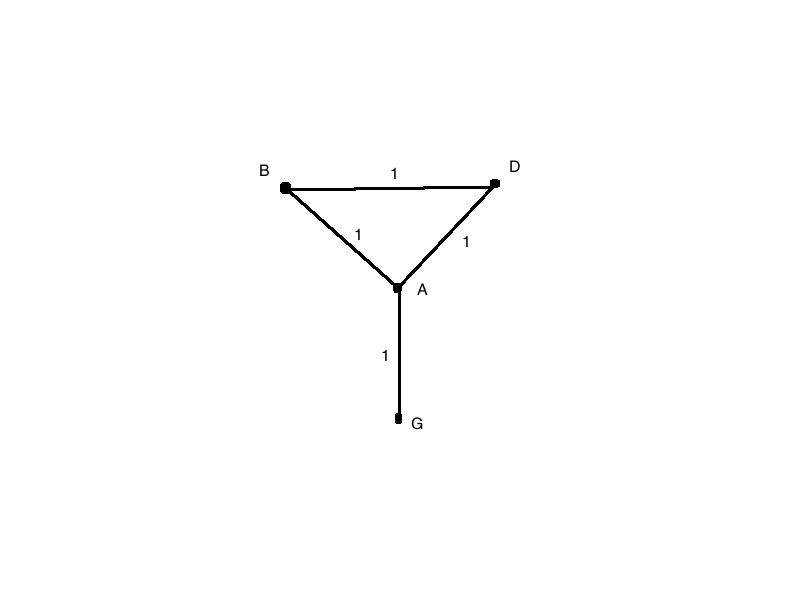
\includegraphics[width=.9\linewidth]{diagrams/counttoinfty.png}

Distance Vector:
\begin{center}
\begin{tabular}{lrrrr}
\hline
DV & A & B & D & G\\
\hline
A & 0 & 1 & 1 & 1\\
B & 1 & 0 & 1 & 2\\
D & 1 & 1 & 0 & 2\\
G & 1 & 2 & 2 & 0\\
\hline
\end{tabular}
\end{center}

\begin{enumerate}
\item Assume link A-G goes down. So, A advertises distance to G=\(\infty\):
A:[0, 1, 1, \(\infty\)]
\item A receives B's DV: A:[0, 1, 1, 3]
\item A sends this DV
\item B recalculates DV: B:[1, 0, 1, 4]
\item This leads to the potential for loops, instability, and long
convergence time
\end{enumerate}

\subsubsection{The Solutions}
\label{sec:orgheadline79}
\begin{enumerate}
\item Set hop/exchange limit to \textbf{16}
\item Split horizon: don't send routes learned from neighbors back to
those neighbors
\item Poison Reverse: Return routes to neighbors set to \(\infty\)
\end{enumerate}

\subsubsection{Routing Information Protocol (RIP)}
\label{sec:orgheadline80}
\begin{itemize}
\item Standard implementation of a DV protocol
\end{itemize}

\subsection{Link State Intra-domain Routing (Djikstra's Algo + Reliable Flooding)}
\label{sec:orgheadline83}
\begin{itemize}
\item Uses Dijkstra's shortest path algorithm to establish forwarding
tables. Assumes link state/costs for all links are available at all
nodes before calculation 

\emph{Assume:}
\begin{enumerate}
\item Each node knows its own link state/cost
\item Each node can communicate with its neighbors
\end{enumerate}
\end{itemize}

\subsubsection{Djistra's Algorithm}
\label{sec:orgheadline82}
N = \# of nodes in G
l(i, j) = link cost between nodes i, j
SPT = nodes comprising shortest path tree
S = source
C(n) = cost of path from S to n
\\
\begin{enumerate}
\item Initialize SPT = \{S\}
for each node not in SPT, C(n) = l(S,n)
\item while(SPT <> N):
SPT = SPT U \{w\} such that C(w) is minimum
for all w in (N-SPT)
\\
for each n in (N-SPT):
C(n) = min(C(n), C(w) + l(w, n))
\end{enumerate}

Ex)
\begin{enumerate}
\item SPT = \{B\}
\item Thus C(E) = 1, C(A) = 3, C(C) = 4, C(others) = \(\infty\)
\item SPT = \{B, E\}, now adjust costs
\item C(A) = min(3, 1+1) = 2\\
C(D) = min(\(\infty\), 1+1) = 2\\
C(F) = min(\(\infty\), )
\end{enumerate}

\section{10/26/17  Cost Metrics, Inter-Domain Routing}
\label{sec:orgheadline92}

\subsection{Quiz 2:}
\label{sec:orgheadline85}

\emph{1.}
Problem = distinguish consecutive strings of 0s and 1s
MRZ, INRZ, Manchester
--
\emph{2.}
RTT = 46.4us = 2Tmax
@ 10Mbps, bit time = 0.1us
Thus, min packet size is 46.4 + 48bits/0.1 = 512 bits
@10Gbps = 46.4 + 48/0.001 = 46,448
Drawback = have to add padding for small data -- inefficient!
--
\emph{3.} 
\begin{enumerate}
\item Switched ethernet builds forwarding tables and makes forwarding
decisions based on these tables
\item No collision domains in switched ethernet, 802.3 requires
collision domains
\end{enumerate}
--
\emph{4.} 
Classes:
A: [0, 7 - Net, 24 - Host]
B: [1, 0, 10 - Net, 16 - Host]
C: [1, 1, 1, 24? - Net, 8 - Host]
Limitations:
\begin{enumerate}
\item inefficient
\item inflexible with respect to routing within a domain
\end{enumerate}
--
\emph{5.} 
   Octagon
\begin{itemize}
\item No distance vectors are exchanged
\end{itemize}

\subsection{Distance Vector Routing}
\label{sec:orgheadline86}
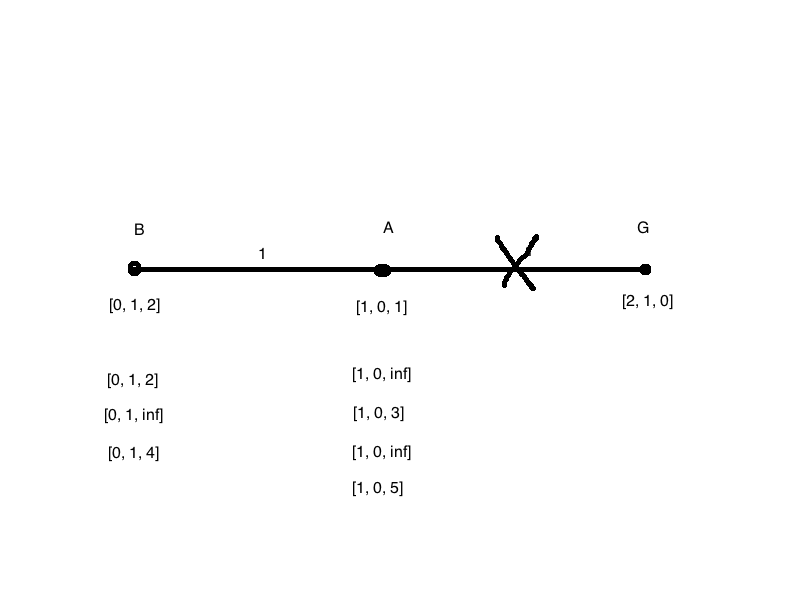
\includegraphics[width=.9\linewidth]{diagrams/fig9.png}
In distance vector routing, whenever you receive an update from a node
that is indicated as the next hop, you may have to raise the cost

\subsection{Link State Routing}
\label{sec:orgheadline89}
\textbf{Link State} = reliable flooding + Dijkstra's
\begin{itemize}
\item In the end, a forwarding table with the next hops is produced
\end{itemize}

\emph{Differences to DV routing:}
\begin{enumerate}
\item Assemble a complete view of the network before executing a routing
protocol
\item Use different protocol (Dijstra's)
\end{enumerate}

\subsubsection{Reliable Flooding}
\label{sec:orgheadline87}
= Process for transmitting link-state packets throughout a network
\begin{itemize}
\item Format: 
\begin{itemize}
\item ID of initiating node
\item List of directly connected nodes
\item Link weights
\item Sequence \#
\item TTL
\end{itemize}

\item Link state change initiates reliable flooding
\begin{enumerate}
\item Initial transmission of link state packets to neighbors
\item Receiving node looks up src/dst record in map table
\item If record \emph{is not} in table, add it and broadcast to all
neighbors (except original neighbor)
\item Else if sequence \# in the table is lower, replace entry and
broadcast
\item Else if sequence \# in table is higher, do nothing
\item Else if sequence \# in table is same, do nothing
\end{enumerate}

\item This enables a consistent view of shortest paths to be established
\item Reliability is enabled by:
\begin{enumerate}
\item Hop by hop acknowledgement of link-state packets
\item Protect update informationin packets via checksum
\item Encryption
\item Remove old (stale) updates via TTL
\end{enumerate}
\end{itemize}

\subsubsection{Open Shortest Path First (OSPF)}
\label{sec:orgheadline88}
= instance of Link State Routing protocol

\begin{itemize}
\item Advantages over RIP: 
\begin{itemize}
\item Fast convergence
\item Loop free routes
\end{itemize}
\item No count to infinity problems - no reliance on neighbor computations
\end{itemize}

\subsection{Link Costs}
\label{sec:orgheadline90}
\begin{itemize}
\item 'Low cost' links are likely to carry traffic

\item Static Metrics (ie. hop(1), \textbf{bandwidth}, distance)
\emph{Pros:} simple
\emph{Cons:} inflexible
\item Dynamic Metrics (ie. latency, packet loss, volume)
\emph{Pros:} adapts to provide better performance
\emph{Cons:} control - complicated to manage

\item Original cost metric: proportional to queue size
\begin{itemize}
\item Problem: Moves packets towards short queues, ignores important
information (ie. bandwidth, latency)
\end{itemize}
\item Next metric: costs proportional to "average delay"

\item In practice, smart configuration of static metrics works about the
same as configuration with dynamic metrics
\begin{itemize}
\item Most administrators prefer static metrics
\end{itemize}
\end{itemize}

\subsection{Inter-domain Routing (Not on midterm)}
\label{sec:orgheadline91}
\begin{itemize}
\item \textbf{Exterior Gateway Protocol} = original inter-domain routing protocol
\begin{itemize}
\item Assumed an "internet backbone"
\end{itemize}

\item Today's internet is organized by interconnections between
\textbf{autonomous systems}
\begin{enumerate}
\item Stub AS = small, single service provider to the rest of the
internet
\item Multi-homed = various sizes, multiple upstream providers
\item Transit = provide local, = size and transit connectivity
\end{enumerate}
\end{itemize}

\section{10/31/17  Border Gateway Protocol}
\label{sec:orgheadline97}
\begin{itemize}
\item Routing tends to be pretty fixed in relatively static networks
\item For Inter-domain routing, there are two objectives:
\begin{enumerate}
\item No loops
\item Policy expression
\end{enumerate}
\end{itemize}
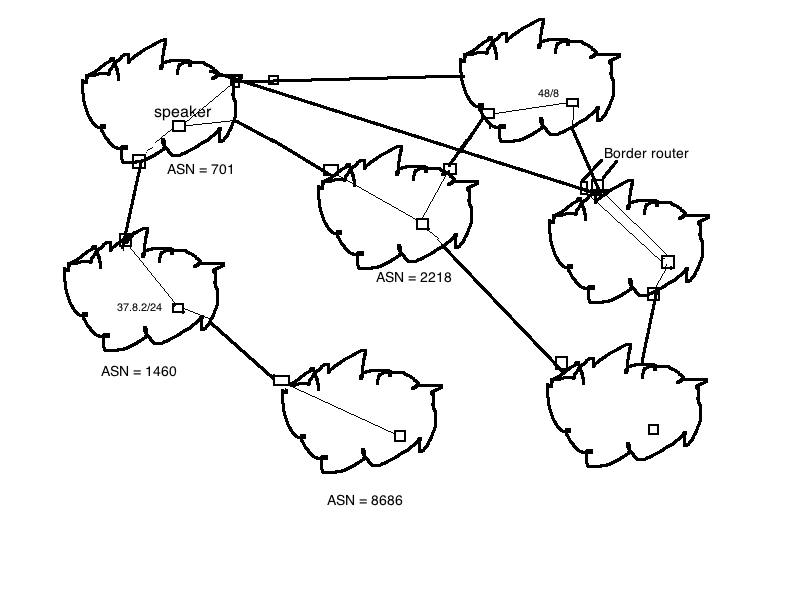
\includegraphics[width=.9\linewidth]{diagrams/bgp1.png}

\subsection{Border Gateway Protocol (BGP)}
\label{sec:orgheadline96}
\begin{itemize}
\item Developed in 1989
\item BGP.4
\item All networks have a \textbf{BGP speaker}
\begin{itemize}
\item A router configured to interact with other BGP speakers in
connected networks. Connections are either:
\begin{enumerate}
\item Customer -\$\$\$-> <-service- Provider
\item Peer, connection is mutually beneficial
\begin{itemize}
\item ie) UW Madison and other Big 10 schools
\end{itemize}
\end{enumerate}
\end{itemize}
\end{itemize}

\subsubsection{Information Exchange}
\label{sec:orgheadline93}
\begin{itemize}
\item Speakers exchange information as follows:
\begin{enumerate}
\item \textbf{Announcing/removing network addresses (uses CIDR)}
\item Transit-only: Announce other reachable networks
\item Full paths and attributes
\begin{itemize}
\item Autonomous System = domain (AS)
\item Full path = sequence of ASNs defined by Path Vector Routing
\end{itemize}
\end{enumerate}

\item Information is exchanged when routes change:
\begin{enumerate}
\item A destination prefix (set of IP addresses) becomes reachable
\item A better path to a prefix becomes available
\item The best path to a prefix becomes unreachable
\item A destination prefix becomes unavailable
\end{enumerate}

\item BGP exchanges are based on Path Vector Routing. Similar to DV
routing, but does not include a provably optimal algorithm for
establishing paths

\item Path vectors are exchanged as follows:
\begin{enumerate}
\item Local network 'announces' the availability of a prefix by
inlcluding the prefix and appending its ASN in a BGP update
packet - send this update to all 'peer' (directly connected)
speakers
\begin{itemize}
\item Ex: path(X (address prefix), ASNY) + policy info
\end{itemize}
\item Peer BGP speaker receive the announcement and then decide how to
proceed -> typical case is to extend path by adding the local ASN
and propogating to peers. -> \emph{path(X, ASNY, ASNZ)}
\item At next AS, path(X, ASNY, ASNZ, ASNA)
\item Loop free routes are ensured by examining the set of ASNs in a
path vector. If you see your own/local ASN in the path, do not
propogate the vector
\end{enumerate}

\item Simple propogation of a path vector is is not the only choice
\begin{itemize}
\item Networks can choose to filter updates
\item Routes can be aggregated via CIDR
\item Propogate a less direct path (in terms of AS hops)
\end{itemize}
\end{itemize}


\subsubsection{Challenges}
\label{sec:orgheadline94}
\begin{enumerate}
\item Number of networks (50k+ networks, 500k+ prefixes)
\item Different interpretations of policy and metrics
\item Need for flexibility
\item Need for trust
\end{enumerate}

\subsubsection{Operation:}
\label{sec:orgheadline95}
\begin{enumerate}
\item Establish session
\item Exchange all active routes
\item Exchange updates
\item Repeat
\end{enumerate}

\section{11/2/17  BGP Control, Multicast}
\label{sec:orgheadline101}
\begin{itemize}
\item BGP is used universally to construct a network of networks
\item Convergence matters in BGP, but there are challenges related to
scale and policy
\item Also, \textbf{path exploration} is standard during updates
\begin{itemize}
\item This refers to intermediate paths that can be used before
convergence
\end{itemize}
\end{itemize}

\subsection{BGP Examples}
\label{sec:orgheadline98}

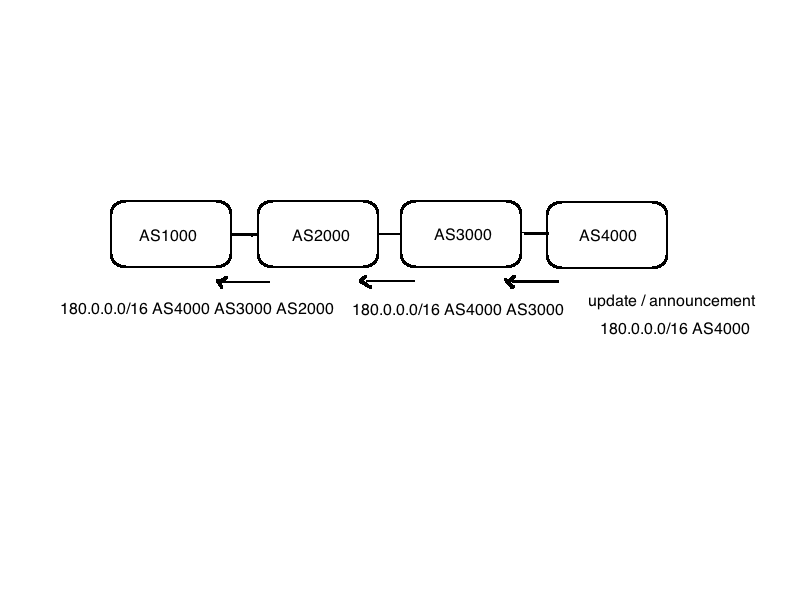
\includegraphics[width=.9\linewidth]{diagrams/bgp2.png}


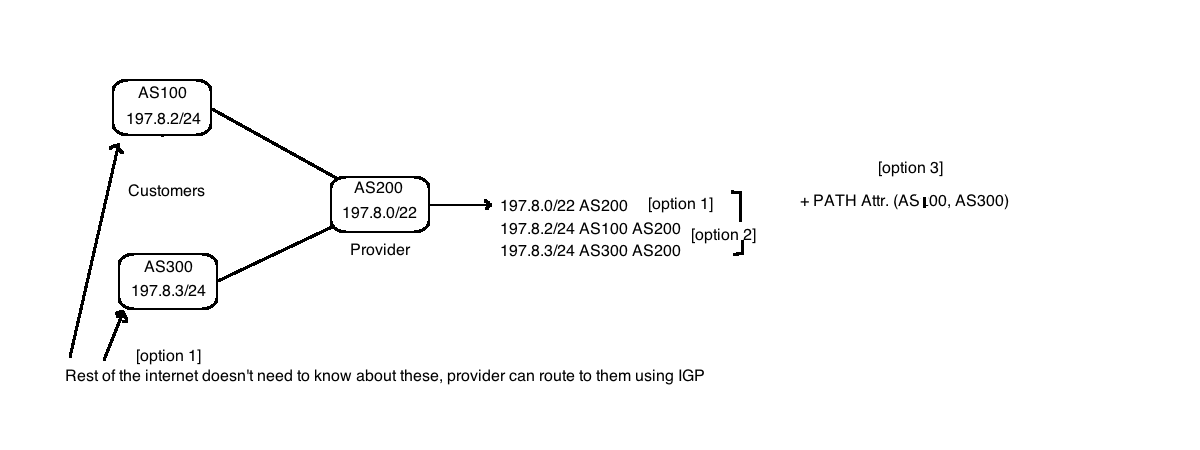
\includegraphics[width=.9\linewidth]{diagrams/bgp3.png}


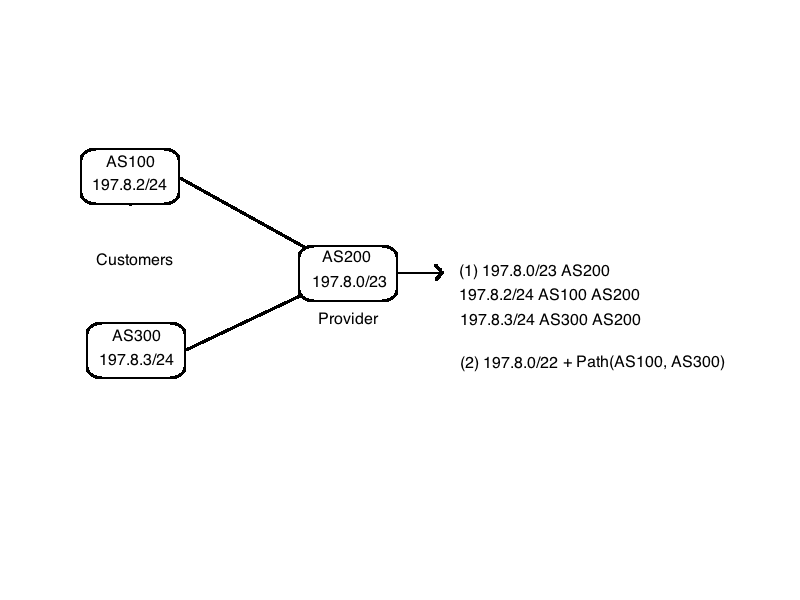
\includegraphics[width=.9\linewidth]{diagrams/bgp4.png}


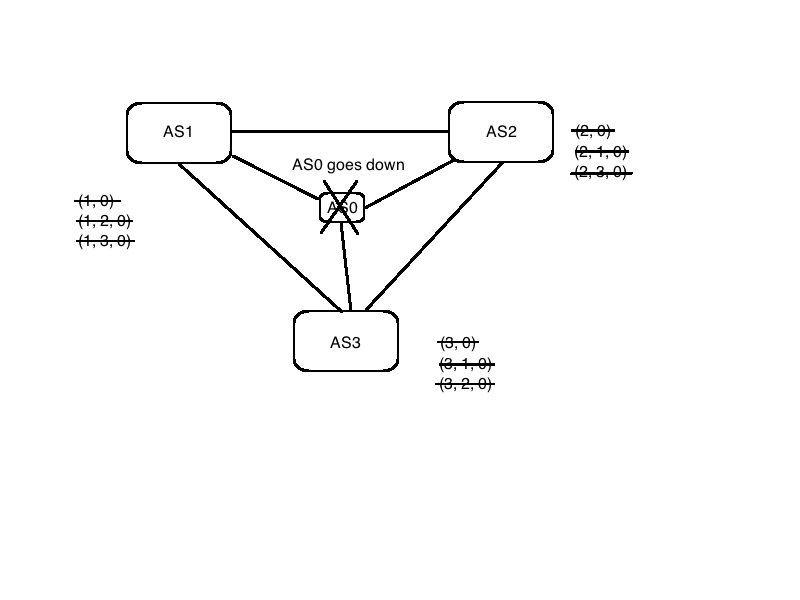
\includegraphics[width=.9\linewidth]{diagrams/bgp5.png}


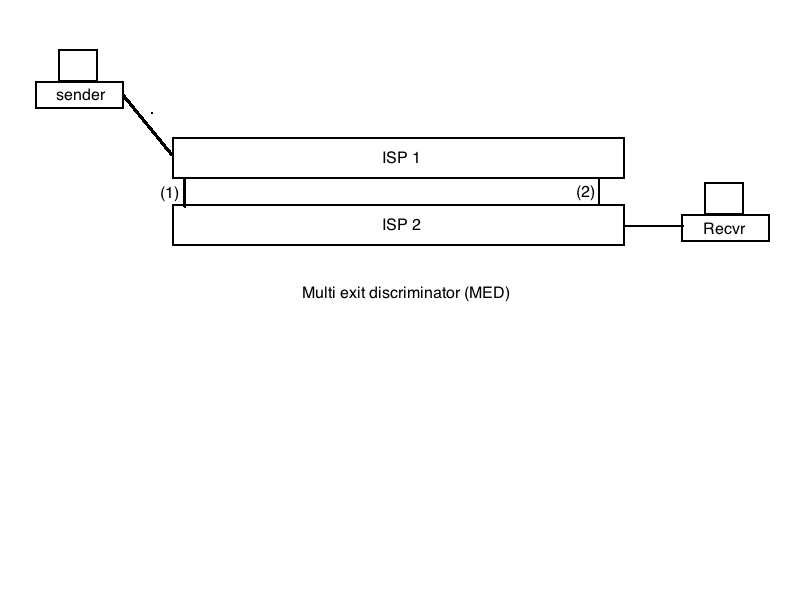
\includegraphics[width=.9\linewidth]{diagrams/bgp6.png}

\subsection{BGP Convergence Times}
\label{sec:orgheadline99}
\begin{itemize}
\item Failover = \textasciitilde{}3min
\item Better path = \textasciitilde{}1min
\item Worse path = \textasciitilde{}2min
\end{itemize}

\subsection{Multicast Routing}
\label{sec:orgheadline100}
\begin{itemize}
\item Observation: 1-to-many communication is inefficient in a unicast
environment (ie. a single connection between server and \emph{each}
receiver)
\end{itemize}

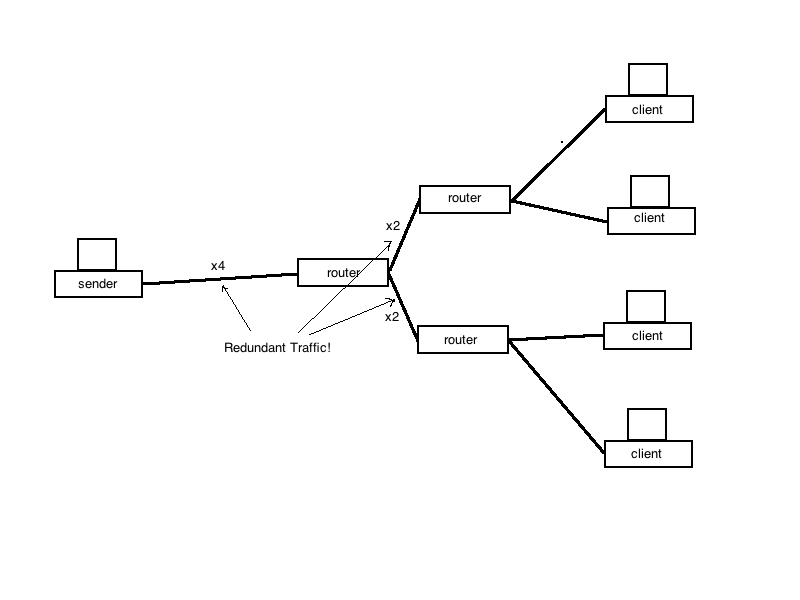
\includegraphics[width=.9\linewidth]{diagrams/multicast.png}

To achieve an efficient transmission of data:
\begin{enumerate}
\item New method for routing
\item A way to duplicate packets
\item New addressing
\end{enumerate}


Multicast routing was invented in 1989 -> RFC1112
\begin{itemize}
\item Senders transmit to a host group i.e. an IP address in the
multicast space
\item Members of a host group = clients that have indicated interest in content
\item Routing must support the connection of senders to receivers
(unicast must also continue to be supported)
\end{itemize}

\textbf{Internet Group Management Protocol (IGMP)} -> clients send IGMP packets
upstream to their first hop router indicating interest in a multicast
host group

\section{11/7/17  Multicast, IPv6}
\label{sec:orgheadline109}
\subsection{Multicast (cont)}
\label{sec:orgheadline102}
\begin{itemize}
\item Clients use \textbf{IGMP} to notify their upstream routers that they want
to receive content from a specific multicast channel (i.e. a multicast
address)
\item Changes in layer 3 infrastructure to support multicast:
\begin{enumerate}
\item IGMP
\item Routers must be able to duplicate packets
\item Mechanism that sets up paths between server and client
\begin{itemize}
\item Protocol + separate multicast forwarding table
\end{itemize}
\end{enumerate}
\end{itemize}

\subsection{Routing Protocol Configuration}
\label{sec:orgheadline103}
\begin{itemize}
\item There are two different configurations that are used in routing
protocols:
\begin{enumerate}
\item Source tree: Root of routing tree is at the server
\begin{itemize}
\item Requires more memory in routers
\item Results in optimal paths
\item Good for situations where you have a small number of
\end{itemize}
senders/large number of receivers
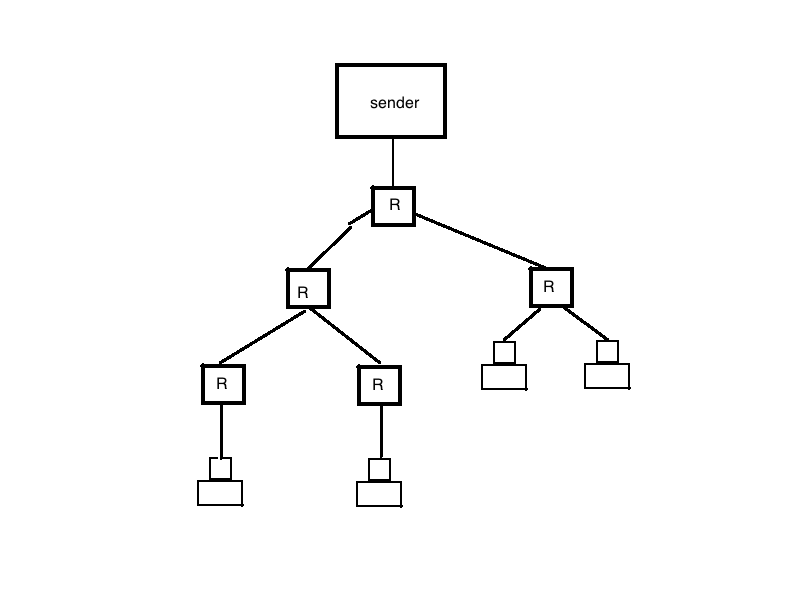
\includegraphics[width=.9\linewidth]{diagrams/sourcetree.png}
\item Shared Tree: Root of routing tree is a special router called a
rendezvous point
\begin{itemize}
\item Requires less memory in routers
\item Can result in suboptimal paths
\item Good for environments with many senders
\end{itemize}
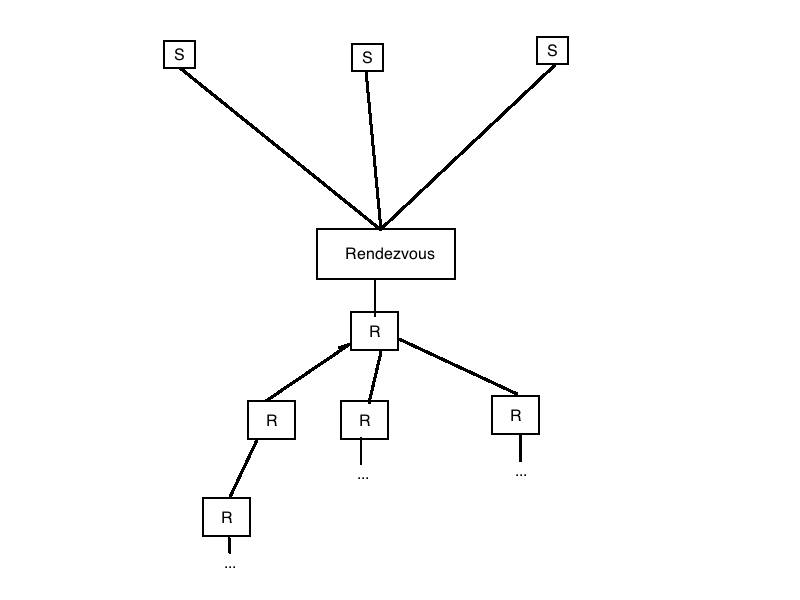
\includegraphics[width=.9\linewidth]{diagrams/sharedtree.png}
\end{enumerate}
\end{itemize}

\subsection{Protocol Independent Multicast (PIM)}
\label{sec:orgheadline107}
\begin{itemize}
\item Assumes that there is an underlying unicast routing protocol
\item PIM operates in dense mode (DM) or sparse mode (SM)
\end{itemize}

\subsubsection{Dense Mode}
\label{sec:orgheadline104}
\begin{itemize}
\item Assumes all clients want to receive content. Clients must opt out
\item Source tree is created via Reverse Path Flooding or via \textbf{Reverse
Path Broadcast}
\end{itemize}

\subsubsection{Reverse Path Broadcast}
\label{sec:orgheadline105}
\begin{itemize}
\item Define parent-child relationships between routers
\end{itemize}
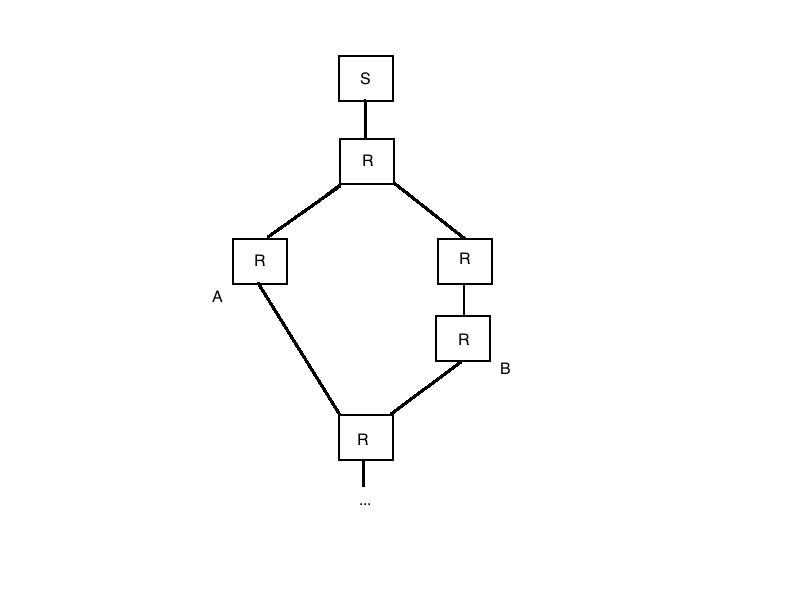
\includegraphics[width=.9\linewidth]{diagrams/rpb.png}
\begin{itemize}
\item R is a parent (ie it is on the forwarding path) if it has a minimum
(lowest cost) path to S. In the example B is not a parent to S so it
will not forward packets in the source tree
\item Requires a global view of the network 
\begin{itemize}
\item Link state routing gives us a global view
\end{itemize}
\item \textbf{SHOULD BE ABLE TO SET UP A SOURCE TREE FOR A NETWORK}
\end{itemize}

\subsubsection{Sparse Mode}
\label{sec:orgheadline106}
\begin{itemize}
\item Assumes clients will opt in on content they want to receive
\item Utilizes a shared tree
\item Requires a \textbf{Rendezvous Point (RP)} which is configured for a set of
servers
\item SM uses "explicit join" to establish paths to the RP. The request
from the client (IGMP) triggers a series of path requests until the
RP is encountered
\end{itemize}

\subsection{IPv6}
\label{sec:orgheadline108}
\begin{itemize}
\item 1991
\item (IPv5 = Internet Stream Protocol, RFC1190)
\item Basic limitation in IPv4 = 32 bit addresses
\item v6 development focused on a number of issues: IPv6 features:
\begin{enumerate}
\item 128-bit addresses
\item Support for real-time QoS (quality of service)
\item Security (IPSEC)
\item Autoconfiguration
\item Enhanced mobility support
\item Multicast support
\item Protocol extensions
\end{enumerate}
\end{itemize}

\section{11/9/17  IPv6, Mobile IP}
\label{sec:orgheadline117}
\subsection{IPv6 Addresses}
\label{sec:orgheadline111}
\begin{itemize}
\item Allocation are classless
\begin{itemize}
\item We continue to use "/" notation
\end{itemize}
\item Standard representation of IPv6 address = 8, 16-bit values separated
by colons
\end{itemize}
Allocations:
\begin{itemize}
\item unicast
\item multicast
\item any cast

\item The IPv6 header was designed to be simpler than IPv4 - fewer fields
and no options. Extension headers enable extra information to be
communicated at layer 3
\item The IPv6 header does \uline{not} include checksum, no header length, no
support for fragmentation
\end{itemize}

\subsubsection{Unicast}
\label{sec:orgheadline110}
\begin{itemize}
\item Indicated by addresses that begin with:
\begin{itemize}
\item 001: There is structure in the remained of the allocation
\begin{itemize}
\item First 64 bits = routing prefix
\begin{itemize}
\item Routing prefix has structure that is meant to reflect the
global network hierarchy. Prefix = Registry, Provier,
Subscriber:
\begin{itemize}
\item Registry = 5-bits
\item Provider = n-bits
\item Subscriber = 56-n bits
\end{itemize}
\item Plus, prefix = 48 bits (or more) of routing/network ID,
followed by 16 bits (or less) of subnet ID
\end{itemize}
\item Followed by 64-bit interface identifier
\end{itemize}
\end{itemize}
\end{itemize}

\subsection{V4 to V6 Transition}
\label{sec:orgheadline112}
\begin{itemize}
\item Native IPv6 requires all routers to support this version of the
protocol in order to transmit packet natively. Otherwise
encapsulation / decapsulation is required
\item BGP for v6 will be required to establish paths. v6 traffic depends
on:
\begin{enumerate}
\item Content providers must make content available on v6
\item Clients must request content on v6
\end{enumerate}
\item Clients now operate "dual stack" hosts. This means that hosts
request \uline{both} v4 and v6 addresses. If both addresses are returned,
host decides which one to use
\end{itemize}

\subsection{Mobile IP}
\label{sec:orgheadline116}
\begin{itemize}
\item RFC 3220
\item IP routing = moving packets from source to destination network. What
if we want to enable hosts to move without changing their IP
address?
\item Mobile IP enables a host to move between networks without having to
change IP addresses
\item Requires changes to infrastructure but not to host
\end{itemize}

\subsubsection{Entities}
\label{sec:orgheadline113}
\begin{itemize}
\item \textbf{Mobile Node (MN)} - Assigned an IP that will not change (from its
home network)
\item \textbf{Home Agent (HA)} - Router in MN's home network. Will forward
packets to MN when it is out of home network
\item \textbf{Foreign Agent (FA)} - Forwards packets to MN when MN is in its
network
\item \textbf{Care-of-Address (CoA)} - Address that identifies the MN's current
location (usually the IP of the FA)
\item \textbf{Correspondent Node (CN)}  - Host that MN is communicating with
\end{itemize}

\subsubsection{Services}
\label{sec:orgheadline114}
\begin{enumerate}
\item Agent discovery: HA and FA announce their presence via ICMP
\item Registration: MN registers its COA from the remote network with the
HA
\item Encapsulation/Decapsulation is used to forward packets from the
home agent to the MN via the COA
\end{enumerate}

\subsubsection{Operation}
\label{sec:orgheadline115}
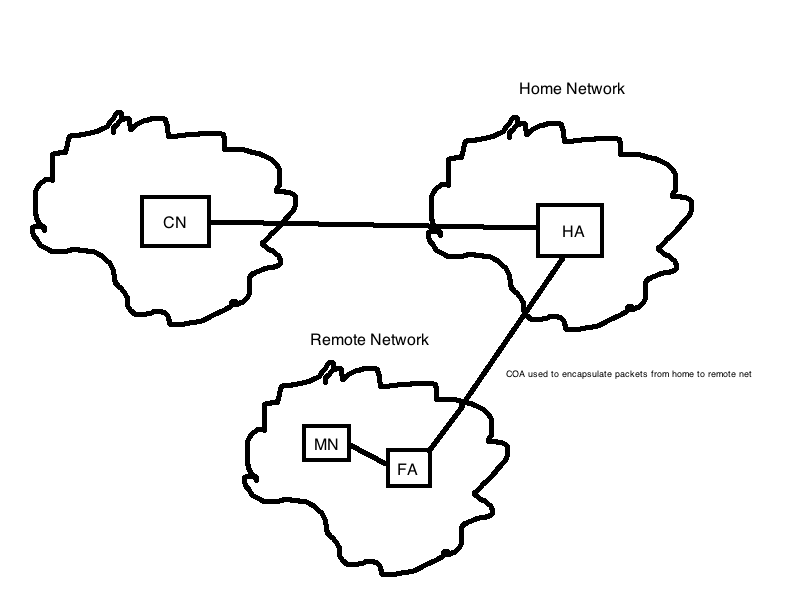
\includegraphics[width=.9\linewidth]{diagrams/mobileip.png}
\begin{enumerate}
\item MN registers with FA wehn it is out of its home net
\item FA forwards req to HA which acknowledges
\item HA then encapsulates all packets sent to MN and fowards via COA
\end{enumerate}

\section{11/14/17 Intro to Transport UDP}
\label{sec:orgheadline124}

\subsection{Issues in Mobile IP}
\label{sec:orgheadline118}
\begin{enumerate}
\item Suboptimal routing
\begin{itemize}
\item Solution: Let the CN know the COA of the MN - in this case the CN
can create its own tunnel to the MN
\end{itemize}
\item Managing placement and operation of Home/Foreign agents in large
networks
\item Frequent movements of clients can lead to significant traffic at
Home Agent
\item \textbf{Security}
\end{enumerate}

\subsection{Transport Layer (4)}
\label{sec:orgheadline119}

\begin{center}
\begin{tabular}{ll}
\hline
(5) & \emph{Many Applications}\\
Transport & < User Datagram Protocol / Transport Control Protocol\\
Network & \\
Data Link & \\
Physical & \\
\hline
\end{tabular}
\end{center}

\begin{itemize}
\item End-to-end connectivity
\item Basic service provided by the transport layer is to multiplex
between multiple applications at Layer 5 and the network at Layer 3
\item Multiplexing is facilitated via \textbf{ports}
\item Because the IP service model is so limited, there are additional
functions that are possible at the transport layer:
\begin{enumerate}
\item Connection control
\item Error detection
\item Reliable delivery
\item In-order delivery
\item Flow control
\item Congestion control
\end{enumerate}
\end{itemize}


\subsection{Layer 4 Multiplexing / Demultiplexing}
\label{sec:orgheadline120}
\begin{itemize}
\item Mux = data is passed from applictation layer down to network layer
\begin{itemize}
\item encapsulate and send to layer 3
\end{itemize}
\item Demux = when packets arrive from layer, examine transport header and
pass up to the appropriate application
\begin{itemize}
\item Ports: 16-bit IDs for both source process and destination
process. Ports 0-1023 = well known < used by servers
\item 1024+ = ephermeral ports < used by clients
\end{itemize}
\end{itemize}

\subsection{Sockets}
\label{sec:orgheadline121}
\begin{itemize}
\item \textbf{Sockets:} Connect applications to the network (sockets "abstract"
the network) by providing a unique handle that associates ports and
processes
\item Socket API defines the creation, attachment, send/receive and close
mechanisms that enable apps to access the network

\item \emph{Create}: required to generate a socket handle that identifies a
network connection
\begin{itemize}
\item int socket(domain (internet), type, protocol(eg. TCP/UDP))
\end{itemize}
\item Next step depends on whether app is a server or a client
\item Assume app is a \emph{server}, so prepare to accept incoming connections
\begin{itemize}
\item int bind(socket, address, addr\(_{\text{len}}\))
\item int listen(socket, backlog)
\item int accept(socket, addr\(_{\text{len}}\))
\item int receive(socket, buffer, buff\(_{\text{len}}\), flags)
\end{itemize}
\end{itemize}

\subsection{User Datagram Protocol (UDP)}
\label{sec:orgheadline123}
\begin{itemize}
\item Simpler, connectionless transport protocol. "datagram" service that
is unreliable/unordered. It provides mux/demux and error detection
(optional for IPv4)
\end{itemize}

\subsubsection{Header}
\label{sec:orgheadline122}
\begin{itemize}
\item 64 bits:
\begin{itemize}
\item 16 bit source port
\item 16 bit destination port
\item 16 bit internet checksum < optional in IPv4, required in IPv6
\item 16 bit length field
\end{itemize}
\end{itemize}

\section{11/16/17 Reliability, TCP}
\label{sec:orgheadline128}
\begin{itemize}
\item UDP packets are "fully defined" by "Destination port/IP pair". ie)
demux is based on this tuple
\end{itemize}

\subsection{Reliable Transport}
\label{sec:orgheadline127}
Goal: Offer a reliable service to applications. This is facilitated by
offering an acknowledgement (ACK) in receipt of a packet.

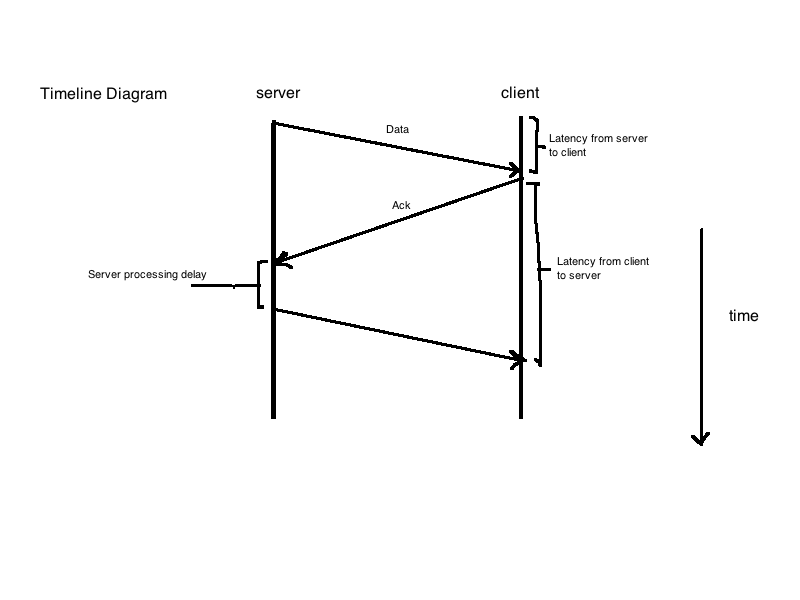
\includegraphics[width=.9\linewidth]{diagrams/timeline.png}

Plus, the server uses a timeout mechanism to decide when to retransmit

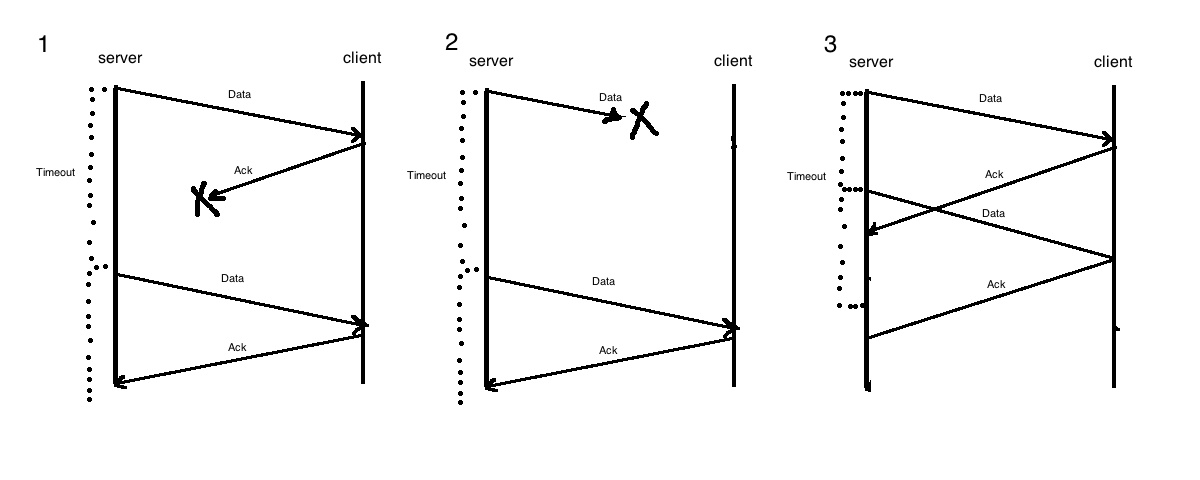
\includegraphics[width=.9\linewidth]{diagrams/timeline2.png}

(Timeout?) Buffers are required on both server and clients

\subsubsection{Timeout/Timers}
\label{sec:orgheadline125}
\begin{itemize}
\item Timeout signals play an important role in reliable transport. If
they are too short, we may resend packets that were not lost
\item If timeout is too long, performance goes down. Goal is to be
sensitive to network conditions
\item Basic mechanism = Exponentially weighted moving average (EWMA) of
RTT from data sent to ACK received
\begin{itemize}
\item Sample RTT is measured for every Data-Ack pair
\end{itemize}
\end{itemize}

\textbf{Equations:}
\[EstRTT = (\alpha * Es) + RTT + (\beta * SampleRTT)\] \\
\[\alpha + \beta = 1\] \\
\[0.8 < \alpha < 0.9\] \\
\[RTO = 2*EstRTT (Retransmit Timeout = RTO)\] \\

\subsubsection{Issues}
\label{sec:orgheadline126}
\begin{itemize}
\item Sending one data packet at a time (ie. waiting for an ACK before
sending the next data packet) may not be an efficient use of network
bandwidth
\item So, to take advantage of network resources, send multiple packets at
a time
\begin{itemize}
\item \emph{Transport decides what to send and when to send it}
\item In UDP this is typically rate-based
\end{itemize}
\item We use "sliding windows" on sender and receiver to improve network
utilization and enable reliability
\begin{itemize}
\item This implies the need to \textbf{flow control} to ensure that the
receiver's buffer is not overflowed. This is a signal that the
receiver sends to the server prior to data flow
\end{itemize}
\item 2 other issues:
\begin{enumerate}
\item The need to identify specific packets -> sequence numbers
\item The need to manage buffers
\end{enumerate}
\item Sequence numbers have an upper limit before wrap around. Basic
requirement:
\[seq num space > num outstanding packets\]
\item Simply stating that seq \# space > \# outstanding packets is
insufficient
\begin{itemize}
\item Assume 3-bit seq \# space ie) seq \#s range from 0-7. 
\begin{enumerate}
\item Sender sends pkts 0\ldots{}6
\item Receiver successfully receives these packets
\item Receiver sends ACKs for all packets, which are lost
\item Sender will resend 0\ldots{}6
\item Receiver expects seq\# \ldots{}7, 0\ldots{}6
\end{enumerate}
\item So, there is a need for a larger seq\# space
\item Max window(send window size) <= (Max Seq\# + 1)/2
\end{itemize}
\end{itemize}

\section{11/21/17 TCP}
\label{sec:orgheadline134}

\subsection{Reliability cont}
\label{sec:orgheadline129}
How to make this efficient for network bandwidth? Send the max window
size as often as possible

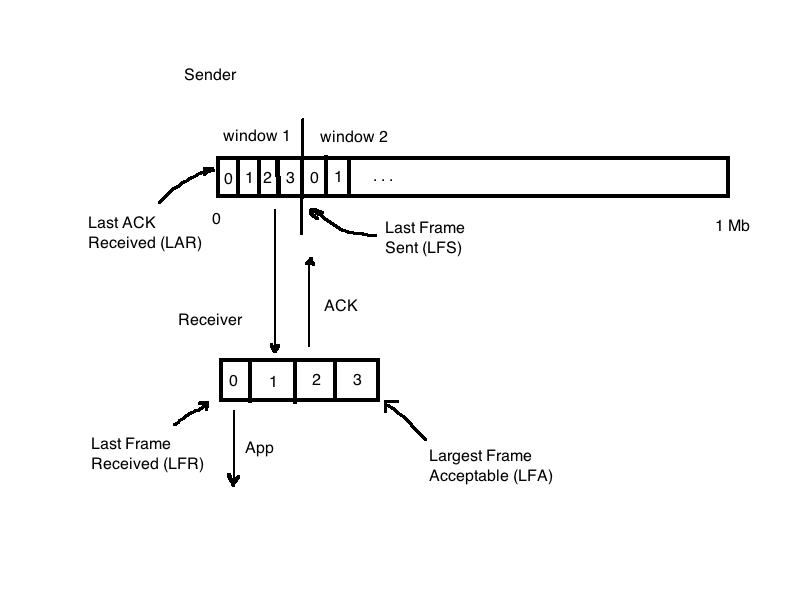
\includegraphics[width=.9\linewidth]{diagrams/flowcontrol.png}

\begin{itemize}
\item Send window size = \textbf{SWS}
\begin{itemize}
\item Upper bound on the \# of unacknowledged packets (in-flight)
\end{itemize}
\end{itemize}

\[LFS - LAR <= SWS\]

\begin{itemize}
\item Sender maintains buffer in order to resend lost packets
\item Receiver maintains buffer to ensure in-order, non-duplicate delivery
to app
\item Receive window size (\textbf{RWS}) = upper bound on out of order frames
\end{itemize}

\[LFA - LAR <= RWS\]

\emph{Implication}: If packet arrives with seq \# < LFR or > LFA, drop that
packet
\begin{itemize}
\item Acks can be "grouped" in a \textbf{cumulative acknowledgement} which ACKs
the sequence number of a group of packets that have successfully
been received
\end{itemize}

\subsection{Transport Control Protocol (TCP)}
\label{sec:orgheadline133}
Features:
\begin{enumerate}
\item Connection oriented
\item Reliable transfer
\item Full duplex
\item Flow control
\item \emph{Byte-oriented}
\item Congestion control
\end{enumerate}

\subsubsection{Header}
\label{sec:orgheadline130}
Features:
\begin{itemize}
\item 16-bit src/dst port \#s
\item 32-bit seq/ack numbers
\item 16-bit checksum
\item 16-bit receive window size
\item Flags: indicate packet type
\begin{itemize}
\item SYN
\item FIN
\item ACK
\end{itemize}
\end{itemize}

\subsubsection{Byte Oriented}
\label{sec:orgheadline131}
\begin{itemize}
\item TCP considers data as an "ordered byte stream" *(except for
congestion control)
\begin{itemize}
\item Implication: Sequence numbers reflect the first byte in a packet
\item Example: Assume a 500KB file with 1 KB maximum segment size and
first byte sequence number = 0. TCP will construct 500 packets
\end{itemize}
\end{itemize}

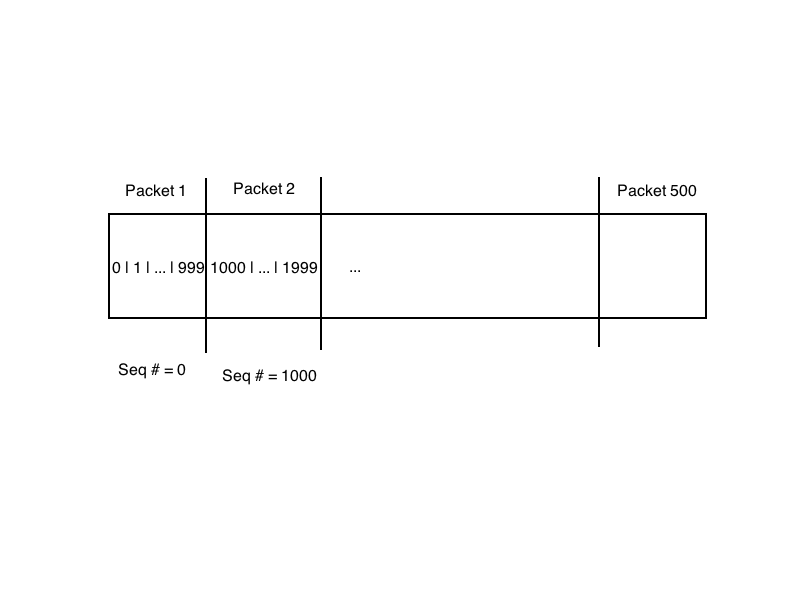
\includegraphics[width=.9\linewidth]{diagrams/TCPex.png}

\begin{itemize}
\item ACKs are a bit tricker. ACKs reflect "the next byte expected". Thus,
the ACK numbers for packets in the example would be:
\begin{itemize}
\item ACK\# for packet 1 = 1000
\item ACK\# for packet 2 = 2000
\end{itemize}
\item Initial sequence numbers are selected randomly by senders
\end{itemize}

\subsubsection{Connection Management}
\label{sec:orgheadline132}
\begin{itemize}
\item See fig 5.7
\item Connections are full duplex that are initiated by \uline{clients}
\item Connections are opened by preamble:
\end{itemize}

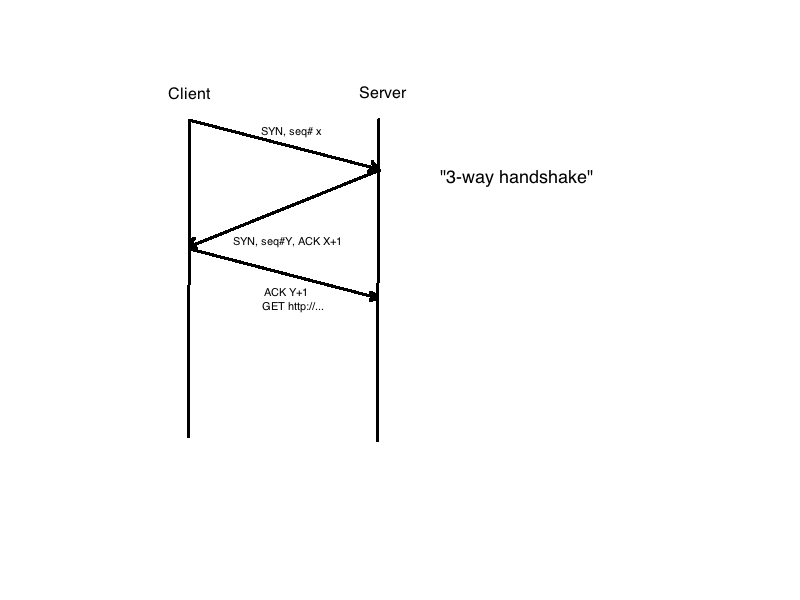
\includegraphics[width=.9\linewidth]{diagrams/connectionmanagement.png}

\begin{itemize}
\item Connections are concluded by an explicit tear-down sequence
\end{itemize}

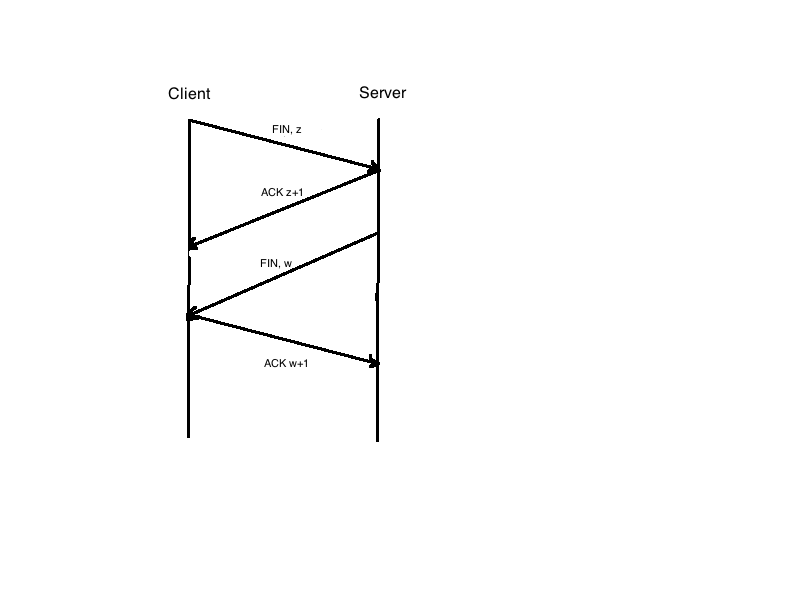
\includegraphics[width=.9\linewidth]{diagrams/teardown.png}

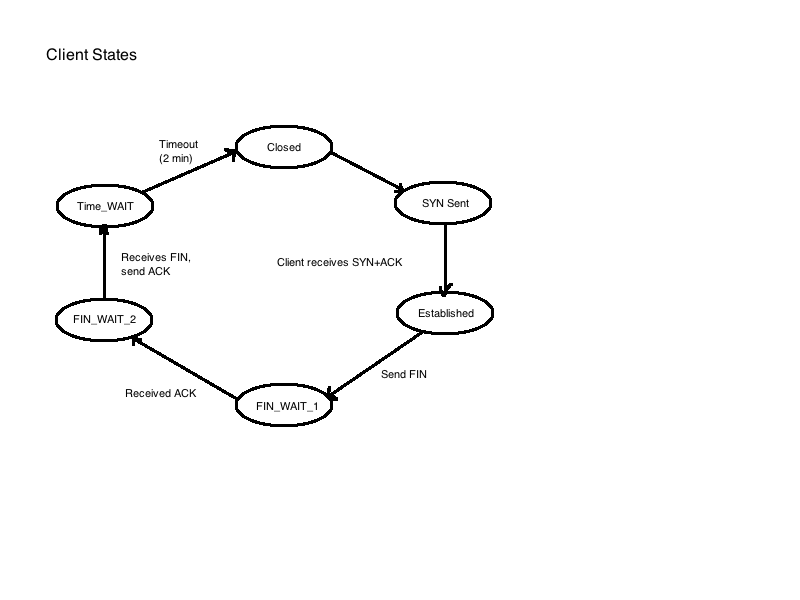
\includegraphics[width=.9\linewidth]{diagrams/clientstates.png}

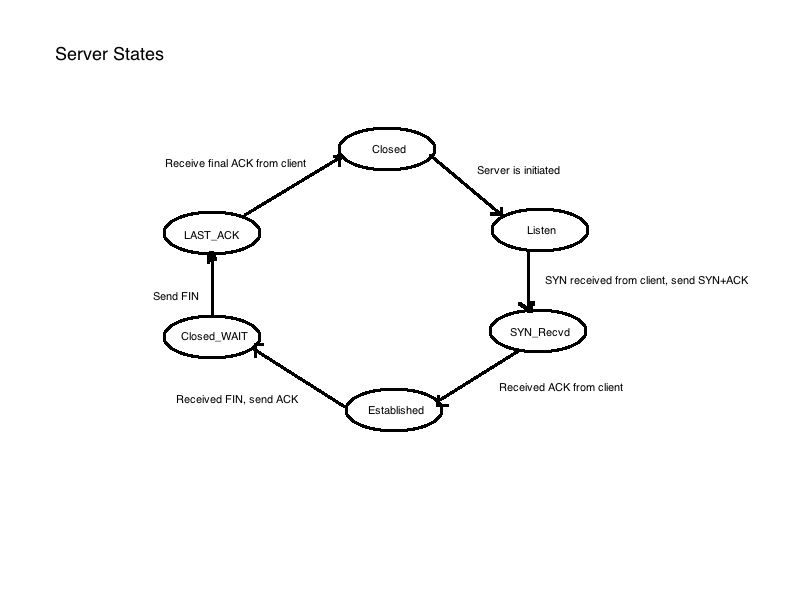
\includegraphics[width=.9\linewidth]{diagrams/serverstates.png}

\section{11/28/17 TCP RTO Calculation, Congestion Control}
\label{sec:orgheadline138}

\subsection{Calculating RTO in TCP}
\label{sec:orgheadline135}
\begin{itemize}
\item How can we improve over basic EWMA?
\begin{enumerate}
\item \textbf{Karn/Partridge algorithm}
\begin{itemize}
\item Don't sample the RTT on lost packets
\item Do exponential backoff on RTO for multiple timeouts
\end{itemize}
\item \textbf{Jacobsen/Karls algorithm} - need to know algorithm

\[Diff = SampleRTT - EstRTT\] \\
\[EstRTT = EstRTT + (d*Diff), 0 < d < 1 (typically ~= 0.125)\] \\
\[Dev = Dev + d * (|Diff| - Dev)\] \\
\[RTO = \mu * EstRTT + \theta * Dev, \mu=1, \theta=4\] \\

\begin{itemize}
\item Sensitive to Sample RTT variance
\end{itemize}
\end{enumerate}
\end{itemize}

\subsection{Congestion Control}
\label{sec:orgheadline137}
\begin{itemize}
\item \textasciitilde{}'87-'89
\item The problem was that at the time, TCP was configured to send a full
window of packets (ie flow control only) whenever possible
\item Congestion control is based on the idea of \textbf{packet conservation}
\begin{itemize}
\item For stability, a host in equilibrium should only inject a new
packet when another packet has been received \emph{(self pacing)}
\end{itemize}
\item TCP Tahoe = original version of TCP with congestion control
\end{itemize}

\subsubsection{Core Mechanism - AIMD}
\label{sec:orgheadline136}
\begin{itemize}
\item Additive increase, multiplicative decrease = \textbf{AIMD}
\item AIMD objective is to be sensitive to the available capactiy of an
end-2-end path
\item TCP Tahoe and subsequent variants use a congestion window (CWND) in
addition to flow control (RWND)
\item CWND limits the number of packets in flight to something less than
RWND
\end{itemize}

\[MaxWindow = min(CWND, RWND)\] \\

\begin{itemize}
\item Increase/decrase CWND depending on capacity of path
\item Adjustments to CWND are based on signals from packets (data/ack) and
in paritcular \emph{loss} (as indicated by RTO)

\item We will grow the size of CWND by probing for additional capacity
\end{itemize}

\uline{Algorithm:}
\begin{enumerate}
\item Increase CWND by 1 for each RTT
\item Decrease CWND by \$\frac{CWND}{2}\& on timeout
\item CWND >= 1
\end{enumerate}


\section{11/30/17 Congestion Control, Congestion Avoidance}
\label{sec:orgheadline144}

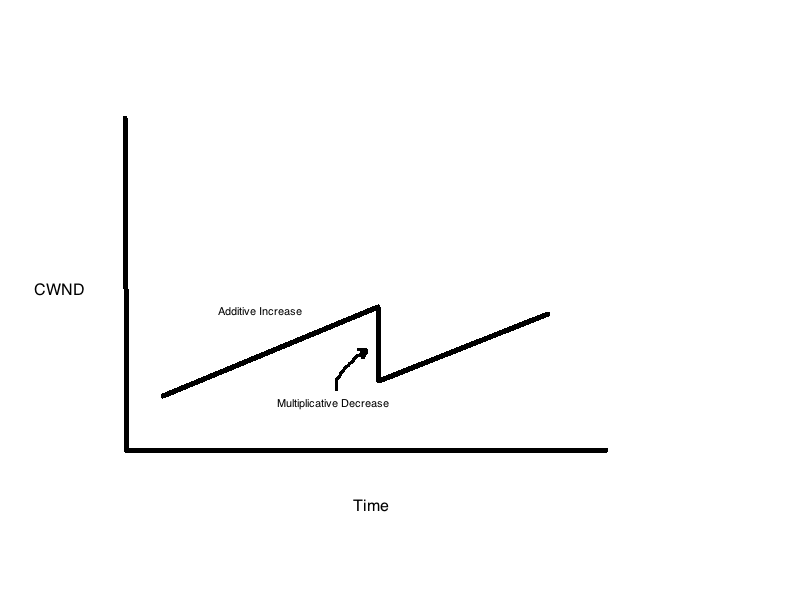
\includegraphics[width=.9\linewidth]{diagrams/AIMD.png}

\subsection{Slow Start in TCP}
\label{sec:orgheadline140}
\begin{itemize}
\item Instead of starting a transfer with a full RWND (ie flow control
limit), start sending at a slower rate, but something faster than
simple additive increase

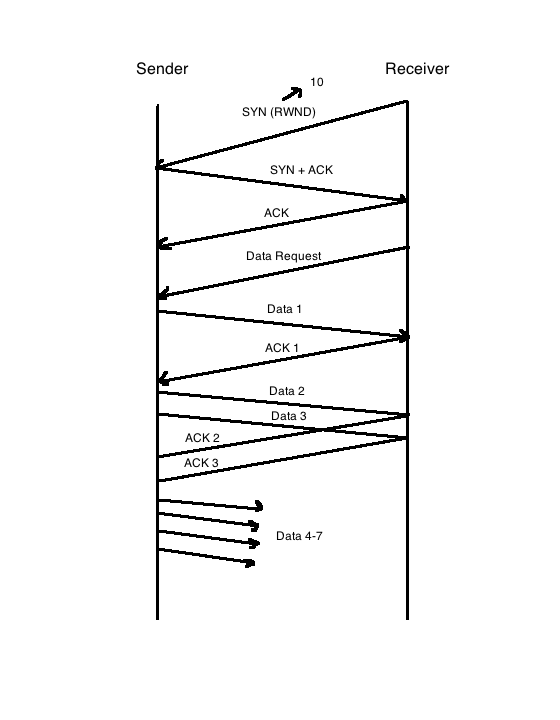
\includegraphics[width=.9\linewidth]{diagrams/SS.png}
\end{itemize}

\subsubsection{Algorithm}
\label{sec:orgheadline139}
\begin{enumerate}
\item Start with CWND = 1
\begin{itemize}
\item Set slow start threshold (SSTHRESH = $\backslash$(inf))lp
\end{itemize}
\item Increase CWND by 1 for each packet acknowledged
\item When CWND >= SSTHRESH when transition to AIMD
\item When at a packet is lost, set SSTHRESH = CWND/2 (for each loss) and
for any loss, set CWND = 1

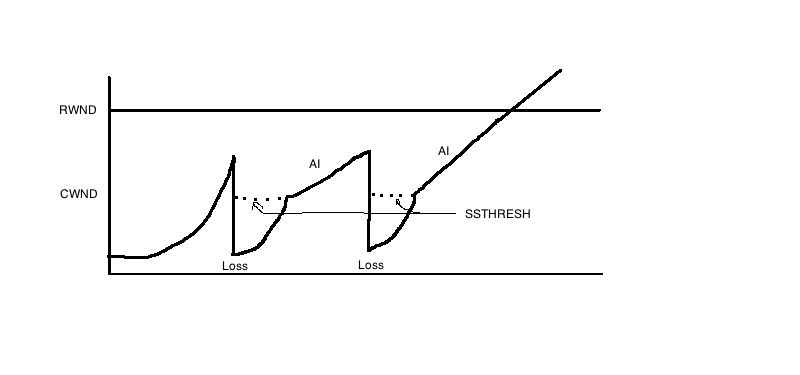
\includegraphics[width=.9\linewidth]{diagrams/SS_2.png}

\begin{itemize}
\item CWND >= 1
\item SSTHRESH >= 2
\end{itemize}
\end{enumerate}

\subsection{TCP Reno}
\label{sec:orgheadline141}
\begin{itemize}
\item Added 2 mechanisms to TCP Tahoe:
\begin{enumerate}
\item Fast Retransmit
\item Fast Recovery
\end{enumerate}
\item Acks returned from receiver can signal that a packet has been lost
\item New signal for last packet:
\begin{itemize}
\item triple duplicate ACK
\end{itemize}
\end{itemize}

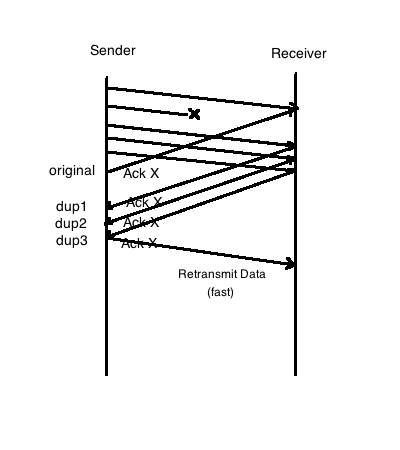
\includegraphics[width=.9\linewidth]{diagrams/Reno.png}

\begin{itemize}
\item \textbf{Fast Retransmit} algorithm:
\begin{enumerate}
\item Upone receipt of 3rd duplicate ACK, retransmit packet that
includes next byte expected
\item After 3rd dup ACK, send one new packet for each ACK received
\end{enumerate}

\item \textbf{Fast Recovery:}
\begin{enumerate}
\item Upon receipt of ACK for lost packet, set SSTHRESH = CWND/2, CWND
= SSTHRESH, Start AI
\end{enumerate}
\end{itemize}

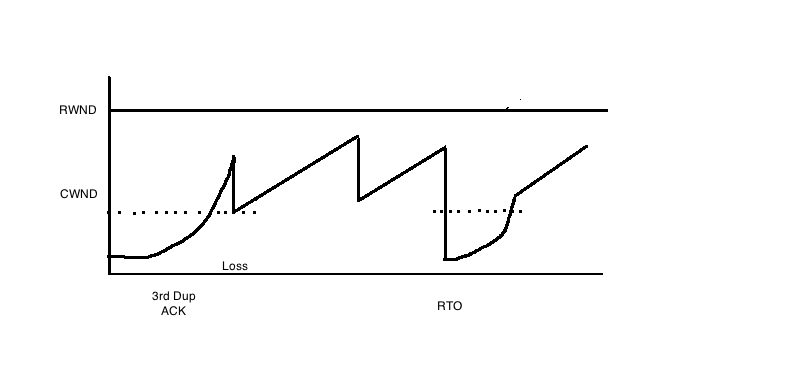
\includegraphics[width=.9\linewidth]{diagrams/Reno_2.png}

\subsection{Congestion Avoidance}
\label{sec:orgheadline143}
\begin{itemize}
\item Instead of designing congestion control that leads to loss, can we
avoid loss all together?
\begin{itemize}
\item Host based: \emph{TCP Vegas}
\item Network based: \emph{Random Early Detection (RED)}
\end{itemize}
\end{itemize}

\subsubsection{TCP Vegas}
\label{sec:orgheadline142}
\begin{itemize}
\item Adjust send rate when there are signals that queues are growing on
an end-to-end path. The signal is that \emph{RTTs grow} (ie send rates go
down)
\item Vegas tries to identify when queues are growing and adjust send rate
to stay just below capacity
\end{itemize}

\uline{Algorithm:}
\begin{itemize}
\item \(Diff = ExpectedRate - ActualRate\) where \(Expected =
  CWND/BaseRTT\)
\item \(ActualRate = CWND/SampleRTT\)
\item If \(Diff < \alpha\) increase CWND linearly. \(\alpha\) is typically = 1
\item If \(Diff > \beta\) decrease CWND linearly. \(\beta\) is typically = 3
\item Else, leave CWND unchanged
\end{itemize}
\textbf{Default behavior for TCP Vegas = TCP Reno when packets are being
lost}

\section{12/5/17 Application Layer}
\label{sec:orgheadline153}

\subsection{Application Architectures}
\label{sec:orgheadline145}
\begin{itemize}
\item Applications run on end hosts - 2 or more are needed
\item Architecture specifies how to organize application on end hosts
\end{itemize}

Architectures:
\begin{enumerate}
\item Client - Server
\begin{itemize}
\item Server: always on and receives and processes requests
\item Clients: sometimes/always on
\item ie) web browsing, email, etc
\end{itemize}
\item Peer-to-Peer (P2P)
\begin{itemize}
\item ie) BitTorrent
\item Arbitrary hosts (peers) communicate directly
\end{itemize}
\item Hybrid
\begin{itemize}
\item Peers communicate directly, but there is also an always on
match-making server
\item ie) Skype, instant messaging
\end{itemize}
\end{enumerate}

\subsection{Application Layer Protocols}
\label{sec:orgheadline146}
\begin{itemize}
\item Protocols specify:
\begin{enumerate}
\item Types: request/response
\item Syntax: field formats
\item Semantics: meaning of fields
\item Rules: for when and how a process sends/receives packets
\end{enumerate}
\end{itemize}

\subsection{The World Wide Web (WWW)}
\label{sec:orgheadline147}
\begin{itemize}
\item Tim Bernes-Lee invented in 1989
\item Organize information into a system of linked documents or objects
\item Components:
\begin{itemize}
\item Structural: Browsers, servers, caches
\item Semantics: HTTP, HTML/XML, URL
\end{itemize}
\end{itemize}

\uline{Browsers:}
\begin{itemize}
\item Run on clients
\item Generate well-formed HTTP requests
\item Interpret HTML data
\item ie) Chrome, Safari, Internet Explorer
\end{itemize}

\uline{Servers:}
\begin{itemize}
\item Wait for requests on port 80 and TCP
\item They house web objects and respond to client requests
\end{itemize}

\uline{Caches:}
\begin{itemize}
\item Copies of frequently requested documents
\end{itemize}

\subsection{HTTP (HyperText Transfer Protocol)}
\label{sec:orgheadline151}
\begin{itemize}
\item Protocol for client/server communication
\item Request: Uniform Resource Location (URL)
\begin{itemize}
\item \url{http://foo.org/index.html}
\end{itemize}
\item 8 different command/reqeust types
\begin{itemize}
\item GET: get the document identified by the URL
\item POST: give information to the server
\item HEAD, PUT, DELETE
\end{itemize}
\item Responses:
\begin{itemize}
\item Status code: 200 OK, 404 not found
\end{itemize}
\item 4 versions:
\begin{itemize}
\item 0.9
\item 1.0
\item 1.1
\item 2.0
\end{itemize}
\end{itemize}

\subsubsection{HTTP 1.0}
\label{sec:orgheadline148}
\begin{itemize}
\item Stop and wait
\item Separate TCP connections for each HTTP request
\item Inefficient:
\begin{enumerate}
\item Latency impact
\item Connection setup and tear down
\end{enumerate}
\end{itemize}

\subsubsection{HTTP 1.1}
\label{sec:orgheadline149}
\begin{itemize}
\item Persistent connection: same TCP with multiple HTTP requests
\item Pipelining: send multiple HTTP requests without waiting for response
\item HOL (head-of-line) blocking - impacts performance
\end{itemize}

\subsubsection{HTTP 2.0}
\label{sec:orgheadline150}
\begin{itemize}
\item Decrease in latency:
\begin{itemize}
\item compression of headers
\item fixed HOL blocking problem
\item server PUSH
\end{itemize}
\end{itemize}

\subsection{Domain Name System (DNS)}
\label{sec:orgheadline152}
\begin{itemize}
\item It is difficult for humans to remember IP addresses
\item DNS resolves names to IP addresses
\item Originally: static list of name-to-IP mapping
\item Hierarchical name space system for internet objects
\begin{itemize}
\item DNS
\end{itemize}
\item Names are read from left to right, separated by periods. Each suffix
in a domain name is a domain
\end{itemize}
ie) cs.wisc.edu
wisc.edu
.edu
\begin{itemize}
\item Port 53 and UDP
\item Rightmost port of domain called Top Level Domain (TLD)
\begin{itemize}
\item Original TLDs: edu, com, gov, mil, org, net
\item Countries: .fr, .uk
\item Arbitrary TLDs
\end{itemize}
\item Top level TLDs managed by ICANN
\end{itemize}

\section{12/7/17 Domain Name System (DNS)}
\label{sec:orgheadline167}
\begin{itemize}
\item Each level of the heirarchy is partitioned into zones
\item Each zone is implemented by 2 or more servers
\item Servers maintain a collection of resource records
\item Types:
\begin{itemize}
\item A = IPv4 address
\item AAAA = IPv6 address
\item NS = name server record
\item MX = mail server
\item CNAME = cannonical name
\end{itemize}
\end{itemize}

\subsection{Content Delivery Network (CDN)}
\label{sec:orgheadline154}
\begin{itemize}
\item Geographically distributed content over a network of proxy servers
and data centers
\item Mechanisms for selecting "best server":
\begin{enumerate}
\item Better performance
\item Reduced latency
\item Load balancing
\item Additional capacity
\end{enumerate}

\item How to pick a CDN server?
\begin{enumerate}
\item Physical proximity
\item Server load
\item Congestion
\item Cheapest path
\end{enumerate}
\end{itemize}

\subsection{Network Security}
\label{sec:orgheadline161}
\subsubsection{Security Services:}
\label{sec:orgheadline155}
\begin{enumerate}
\item Privacy: Prevent unauthorized access to data
\item Authentication: Verifying ID of remote user
\item Integrity: Make sure messages have not been altered = assurance
that information is trustworthy
\item Confidentiality: Encrypt messages to prevent adversary from
understanding messages
\begin{itemize}
\item Traffic confidentiality: concealing the quantity of traffic on
destination
\end{itemize}
\end{enumerate}

\subsubsection{Symmetric-Key Encryption}
\label{sec:orgheadline156}
\begin{itemize}
\item Sender and receiver share the same "secret key"
\item Data Encryption Standard (DES)
\begin{itemize}
\item 56-bit keys
\item 2\(^{\text{56}}\) search space for keys
\item because of parallelism DES became unusable
\end{itemize}
\item 3-DES
\begin{itemize}
\item 168-bit keys
\end{itemize}
\item Advanced Encryption Standard (ADS)
\begin{itemize}
\item 128, 192, or 256 bits
\end{itemize}
\end{itemize}

\subsubsection{Public Key Ciphers}
\label{sec:orgheadline157}
\begin{itemize}
\item Pair of keys owned by one participant
\item Decryption using "private key"
\item Encryption using "public key" -> shared
\item Ex) Riverst Shamir Adlemann (RSA)
\begin{itemize}
\item Keys are products of 2 large prime numbers
\item 1024 bits
\item High computational cost of factoring large prime numbers
\end{itemize}
\end{itemize}

\subsubsection{Key Exchange}
\label{sec:orgheadline158}
\begin{itemize}
\item Diffie-Hellman Key Exchange
\item RSA tokens
\end{itemize}

\subsubsection{Data Integrity}
\label{sec:orgheadline159}
\begin{itemize}
\item Encryption does not guarantee data integrity since random bit flips
can result in a plain text message that looks valid
\item To address integrity and to prevent tampering of messages, we use
"redundancy", \textbf{cryptographic checksum}
\item To do this, we use "cryptographic has function"
\item Output = Message Digest (MD)
\begin{itemize}
\item MDs have special property that they produce some number of bits
regardless of length of message
\end{itemize}
\end{itemize}

\subsubsection{Authentication}
\label{sec:orgheadline160}
\begin{itemize}
\item Note as simple as appending signatures to every message
\item Replay and delayed-replay attacks
\begin{itemize}
\item ex) credit card online purchase (replay), stock market, auction
(delayed-replay)
\end{itemize}
\item Use "session-keys" = symmetric-key ciphers
\end{itemize}

\subsection{Challenge Response Protocol}
\label{sec:orgheadline162}
\begin{itemize}
\item Simple one-way authentication protocol
\end{itemize}

\subsection{Public Key Authentication}
\label{sec:orgheadline165}
(assuming clock synchronization)
\subsubsection{Public Key Auth (without clock sync)}
\label{sec:orgheadline163}
\subsubsection{Kerberos}
\label{sec:orgheadline164}
\begin{itemize}
\item Trusted 3rd party with whom hosts share keys
\item via 3rd party auth sequence is initiated
\end{itemize}

\subsection{Issues in Security}
\label{sec:orgheadline166}
\begin{itemize}
\item Threat models = how exactly bad guys attack?
\item Key distribution = Public Key Infrastructure (PKI)
\item Verification = how can we be sure systems are secure?
\end{itemize}


\section{12/12/17 RED, Network Security}
\label{sec:orgheadline171}
\subsection{Congestion Avoidance}
\label{sec:orgheadline169}
\begin{itemize}
\item Host-based = TCP Vegas
\begin{itemize}
\item Adjust CWND to pay attention to sending rate and building queues
\item Never deployed
\end{itemize}
\item Network-based = \textbf{RED} (Random Early Detection)
\begin{itemize}
\item Intuition behind RED: have the network notify senders when
congestion is building
\begin{itemize}
\item Explicit Congestion Notification (\textbf{ECN})
\item Implicity -> drop (same) packet \textbf{*}
\end{itemize}
\end{itemize}
\end{itemize}

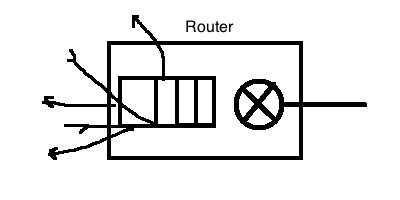
\includegraphics[width=.9\linewidth]{diagrams/router_congestion.png}

\subsubsection{RED Algorithm}
\label{sec:orgheadline168}

\(AvgQueueLen = (1 - w) * AvgQueueLength + (w * SampleQueueLength),
w~=0.002\) \\

\begin{itemize}
\item If AvgQueueLength <= MinThreshold
\begin{itemize}
\item Enqueue packet
\end{itemize}
\item If MinThreshold < AvgQueueLength < MaxThreshold
\begin{itemize}
\item Calculate p
\item Drop next packet with probability = p
\end{itemize}
\item If AvgQueueLength >= MaxThreshold
\begin{itemize}
\item Drop next packet
\end{itemize}
\end{itemize}

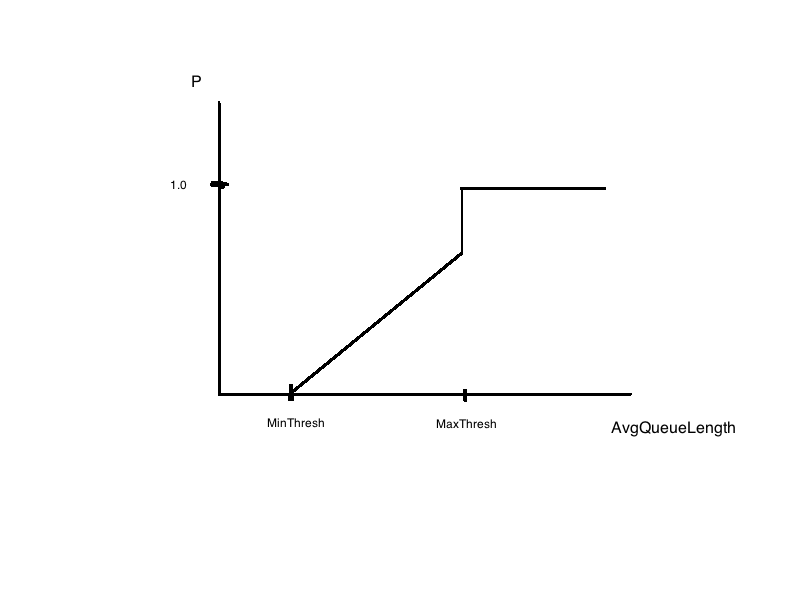
\includegraphics[width=.9\linewidth]{diagrams/RED.png}

\subsection{Network Security}
\label{sec:orgheadline170}
\begin{itemize}
\item Key Issue: Addressing threats/adversaries. Motivations:
\begin{itemize}
\item \$\$\$
\item Recognition
\item "Terrorism" (Nation-state activities)
\end{itemize}
\item How are attacks facilitated?
\begin{itemize}
\item Security is not part of Internet architecture!
\item Open Internet model
\item Inversion of work
\item Anonymity
\item Complexity
\item Humans in the loop
\end{itemize}
\end{itemize}
\end{document}